% CVPR 2026 Paper Template; see https://github.com/cvpr-org/author-kit

\documentclass[10pt,twocolumn,letterpaper]{article}

%%%%%%%%% PAPER TYPE  - PLEASE UPDATE FOR FINAL VERSION
% \usepackage{cvpr}              % To produce the CAMERA-READY version
\usepackage[review]{cvpr}      % To produce the REVIEW version
% \usepackage[pagenumbers]{cvpr} % To force page numbers, e.g. for an arXiv version

% Import additional packages in the preamble file, before hyperref
\input{preamble}
\usepackage{graphicx}
% Per [D-45] master-source architecture: figures live in papers/shared/figures;
% the {../shared/} prefix lets sec/*.tex use \includegraphics{figures/<name>} unchanged.
\graphicspath{{../shared/}}
\usepackage{tikz}
\usetikzlibrary{positioning, arrows.meta, shapes.geometric, backgrounds}

% Per [D-45]: canonical numerical chokepoint (single source of truth for result-claim numerals)
% papers/shared/numbers.tex
% Canonical numerical chokepoint per [D-45] master-source architecture.
%
% Rule (per [D-45]): result-claim sentences in papers/shared/sec/*.tex
% should cite \newcommand{}s defined here rather than bare numerals,
% so that a single update propagates across all venue manifests.
%
% This file is currently empty. The numbers.tex bootstrap sprint
% will populate it with macros for the [D-44] bootstrap values,
% the τ-binned R range, the P_F failure range, etc. See
% experiments/nerf/LEDGER.md §3 [D-45] for the full schema spec.
%
% Until populated, atoms continue to use inline numerals;
% this file's existence is the architectural seed, not the
% finished chokepoint.



% It is strongly recommended to use hyperref, especially for the review version.
% hyperref with option pagebackref eases the reviewers' job.
% Please disable hyperref *only* if you encounter grave issues, 
% e.g. with the file validation for the camera-ready version.
%
% If you comment hyperref and then uncomment it, you should delete *.aux before re-running LaTeX.
% (Or just hit 'q' on the first LaTeX run, let it finish, and you should be clear).
\definecolor{cvprblue}{rgb}{0.21,0.49,0.74}
\usepackage[pagebackref,breaklinks,colorlinks,allcolors=cvprblue]{hyperref}

%%%%%%%%% PAPER ID  - PLEASE UPDATE
\def\paperID{*****} % *** Enter the Paper ID here
\def\confName{CVPR}
\def\confYear{2026}

%%%%%%%%% TITLE - PLEASE UPDATE
\title{CosmoGasVision: 3D Intergalactic Medium Reconstruction via Implicit Neural Representations}

%%%%%%%%% AUTHORS - PLEASE UPDATE
\author{Anonymous CVPR submission}

\begin{document}
\maketitle

\begin{abstract}
Reconstructing the three-dimensional (3D) distribution of the intergalactic medium (IGM) from sparse one-dimensional (1D) Lyman-alpha forest sightlines is a sparse-view tomography problem with a physically derived forward operator. Classical voxel-grid methods such as TARDIS~\cite{horowitz2019tardis} and Wiener filtering~\cite{stark2015tomography} discretize the volume up front, trading resolution for memory or memory for spectral aliasing.

We present \emph{CosmoGasVision}, a continuous neural field $F_\theta:\mathbf{x} \to (\rho, T, X_{HI}, v_{\text{pec}})$ optimized end-to-end against a fully differentiable Lyman-alpha optical-depth integrator. The integrator implements the Tepper-Garc\'ia~\cite{tepper2006voigt} analytic Voigt-Hjerting kernel, full redshift-space-distortion (RSD) convolution, a learnable amplitude that absorbs absolute calibration constants, a saturated-absorber mask~\cite{wolfe2005}, and a mean-flux soft anchor at the verified value $\langle F\rangle_{\text{obs}}(z=0.3) = 0.979 \pm 0.005$~\cite{kirkman2007}.

At the corrected anchor and full publication schedule (\texttt{pub-t1}, $50{,}000$ steps, four Sherwood~\cite{bolton2017sherwood} feedback variants $P_1$--$P_4$, seed $=0$), \emph{two of three} primary [D-13] gates close at the single-seed level: mean-flux closes $4/4$ at the seed=42 single-seed anchor (cross-physics spread $0.63\%$, $<\!1\%$ bar), but a 5-seed sightline-level bootstrap shows the population CI overlaps the Kirkman+2007 anchor $[0.974, 0.984]$ in only $2/4$ cells ($P_3$ and $P_4$ marginal at q84); $P_1$ and $P_2$ bootstrap CIs sit entirely below the anchor band. The flux-PDF Kolmogorov--Smirnov gate closes $3/4$ bootstrap-robustly. The binding gate fails: the 1D flux-power-spectrum residual $|\Delta P_F/P_F|$ over the inertial range $k_\parallel \in [10^{-2.5}, 10^{-1.5}]$ s/km remains $36\%$--$42\%$ in $4/4$ cells, $3.6$--$4.2\times$ over the $10\%$ bar. A $\tau$-binned residual decomposition cross-physics positively identifies saturation-regime under-fitting ($F \in [0.05, 0.30]$) as the residually-supported mechanism (concentration ratio $R \in [18.87, 23.75]$, $>\!12\times$ over the positive-ID floor in $4/4$ cells). Three counterfactual interventions against this mechanism --- a saturation-aware $P_F$ band loss, an FGPA-tail per-pixel regularizer, and velocity-gradient conditioning --- each failed by a previously-unaudited degeneracy class, retired under pre-committed stop conditions.

The contributions are (i) a continuous-neural-field formulation of Ly$\alpha$ tomography coupled to a differentiable Voigt integrator, with a cost-survey-validated linear-VRAM training schedule across feedback physics; (ii) the calibration-vs-structure falsification that surfaces $P_F$ --- not anchor calibration, not sightline density alone --- as the binding gate, with the deficit residually localized to the saturation band cross-physics; (iii) a falsification-disciplined methodology of pre-committed gates and degeneracy-aware counterfactuals that converts negative results into successor-experiment constraints. We do not claim to have solved 3D IGM reconstruction; we report a partial result with the binding obstacle named.
\end{abstract}

\section{Introduction}
\label{sec:intro}

This paper is, in computer-vision language, a sparse-view tomography problem with an unusual sensing modality. The volume to be reconstructed is the \textbf{intergalactic medium} (IGM) --- the diffuse gas filling the space between galaxies, which holds the majority of the universe's ordinary (baryonic) matter and forms the filaments and voids of the \emph{cosmic web}. We have no camera that can image this volume directly. Instead, we observe it through \textbf{Lyman-alpha forest} spectra: when light from a distant quasar passes through the IGM on its way to Earth, neutral hydrogen along the path absorbs photons at a specific resonance wavelength, and Doppler shifts caused by cosmic expansion smear that absorption into a dense forest of narrow dips across the quasar's spectrum. Each such 1D spectrum is a \textbf{sightline}: a single ray through the cosmological volume --- the analogue of one CT scanline through a body, or one pixel column in a 3D scan --- and the position of every absorption dip encodes the gas state at one location along that ray.

Reconstructing the 3D IGM from a sparse bundle of such 1D sightlines is therefore literally tomography from pencil-beam projections, referred to as \emph{Lyman-alpha tomography}~\cite{stark2015tomography} in astrophysics and as sparse-view inverse rendering with a known forward operator in CV vocabulary. Classical solutions like TARDIS~\cite{horowitz2019tardis} and Wiener filtering~\cite{stark2015tomography} discretize the volume into a fixed voxel grid; at the typical inter-sightline spacing of survey data (several $h^{-1}$ Mpc transverse), this either over-commits memory or aliases the small-scale absorption structure that the metrics actually care about.

\textbf{Motivation.} Neural Radiance Fields (NeRF)~\cite{mildenhall2020nerf} replaced explicit voxel grids in vision with a coordinate-conditioned MLP, supervised through a differentiable rendering integral. The same representational move is what the IGM problem needs. We are not interested in rendering visual color; we are interested in recovering an underlying physical state from absorption profiles, and we want a representation whose gradient flows cleanly through the forward physics rather than getting interrupted by a discretization seam.

\textbf{Contribution.} We introduce \emph{CosmoGasVision}, a NeRF-style continuous field for cosmological gas, coupled to a custom differentiable projector that maps the MLP-decoded physical fields to 1D Lyman-alpha optical depth (a logarithmic measure of light absorbed along the sightline; see \cref{sec:method}) using the analytic Voigt-Hjerting kernel~\cite{tepper2006voigt}. The contribution is the representation-plus-forward-model package: a continuous IGM field optimized end-to-end against the same physics that astrophysicists already trust, so that recovered structures are sub-voxel in resolution while every step of the gradient path remains physically interpretable.

\textbf{What this paper is, and is not.} This paper does not demonstrate a closed-loop 3D IGM tomography from sparse Ly$\alpha$ sightlines. At the corrected anchor and full publication schedule, two of three primary [D-13] structure gates close at the single-seed level (mean-flux $4/4$ at seed=42, bootstrap $2/4$ at the population CI; KS $3/4$) while the binding inertial-range $P_F$ residual fails $4/4$ at $\PFfactorOverGateLo\times$--$\PFfactorOverGateHi\times$ the gate. A $\tau$-binned residual decomposition positively localizes the saturation band $F \in [\SatBandLo, \SatBandHi]$ as the residually-supported mechanism cross-physics; three counterfactual interventions tested under the [D-37] discipline retire under previously-unaudited degeneracy classes. The remaining gap is therefore residually supported but not closed.

\textbf{What this paper is.} (i) A continuous-neural-field formulation of Ly$\alpha$ tomography with a differentiable RSD-convolved Voigt integrator, a saturated-absorber mask, and a mean-flux soft anchor at the verified low-$z$ value~\cite{kirkman2007}; (ii) a cost-survey-validated training schedule with a closed-form linear-VRAM model across feedback physics and sightline-density tiers; (iii) a calibration-vs-structure falsification that surfaces $P_F$ --- not anchor calibration, not sightline density alone --- as the binding gate, with the deficit residually localized to the saturation band cross-physics; (iv) a falsification-disciplined methodology of pre-committed structure gates, degeneracy-aware counterfactuals, and pre-committed stop conditions on each counterfactual, so negative results become explicit constraints on the successor design rather than discarded attempts.

The canonical classical IGM-tomography baselines are TARDIS~\cite{horowitz2019tardis} (Bayesian Wiener-filter reconstruction) and Stark+ Wiener filtering~\cite{stark2015tomography}. We position our continuous-neural-field formulation against these as qualitative comparison; a numerical reproduction of either is out of scope for the present paper.

\section{Related Work} % Project Foundation: Background for Stages 1-3
\label{sec:related}

\textbf{Cosmological Ly$\alpha$ tomography.} The reconstruction of the 3D IGM from sparse Ly$\alpha$ forest sightlines has a $\sim\!25$-year methodological history. Pichon et al.~\cite{pichon2001tomography} cast the inversion as a nearest-neighbor / Wiener-style filter on quasar sightlines, establishing the voxel-grid framing that the modern era inherited. Stark et al.~\cite{stark2015tomography} formalized the sparse-tomography setting at $z \sim 2.3$ and demonstrated Wiener-filter reconstruction at survey-realistic inter-sightline spacing; Horowitz et al.~\cite{horowitz2019tardis} introduced TARDIS, a constrained-optimization scheme that absorbs absorption-line physics directly into the inverse-problem objective. Lee et al.~\cite{lee2015, lee2018clamato} consolidated the observational requirements and first-light realization of the CLAMATO survey at $z\sim 2.3$. These are the comparison points for any continuous-representation work at low redshift. They share a common design choice --- an explicit voxel grid as the reconstruction primitive --- which the present work substitutes with a continuous coordinate-conditioned MLP.

\textbf{Implicit neural representations.} In computer vision, NeRF~\cite{mildenhall2020nerf} initiated a wave of coordinate-based MLP scene representations supervised through a differentiable rendering integral. The bandwidth of the input encoding turns out to control representable spatial frequency in a precise way that Tancik et al.~\cite{tancik2020fourier} characterize for Fourier features; SIREN~\cite{sitzmann2020siren} extends the same idea with periodic activations throughout the MLP, with sharper-than-ReLU spectral profiles on high-frequency targets. The representation has been ported beyond static scenes: NeRV~\cite{chen2021nerv} represents whole videos as a single coordinate-conditioned MLP, and Instant NGP~\cite{muller2022instant} uses a multiresolution hash grid to accelerate the same family of architectures by orders of magnitude. We adopt Fourier positional encoding at $L=10$ as our bandwidth selector (Sec.~\ref{sec:method}); the higher-bandwidth-without-grid alternatives of~\cite{sitzmann2020siren, muller2022instant} are open ablation axes for the successor design.

\textbf{Physics-informed neural networks.} The introduction of physical constraints into neural-network optimization --- typically as soft penalty terms enforcing PDE residuals --- is the PINN framework of Raissi et al.~\cite{raissi2019pinn}, surveyed in Karniadakis et al.~\cite{karniadakis2021pinns}. Our setup is structurally related but operationally distinct: rather than penalizing residuals of a governing equation, we propagate gradients through a complete physical forward model (the RSD-convolved Voigt-Hjerting kernel, Sec.~\ref{sec:method}) and supervise against an observable that is the model's natural output. The FGPA $\tau \propto \rho^{1.6} T^{-0.7}$~\cite{bi_davidsen1997, hui_gnedin1997} is the analogous PDE-residual prior in our domain; it figures in the successor-work design (Sec.~\ref{sec:nextsteps:pf} \#1) but is not a load-bearing component of the present model. Earlier cosmological ML work used CNN and GAN architectures over voxelized inputs~\cite{zamudio2019higan, ravanbakhsh2017cosmology} without coupling to a differentiable observational operator.

\textbf{Sparse-view inverse rendering in medical imaging.} The closest cross-domain analogue of our problem is sparse-view cone-beam computed tomography (CBCT) reconstructed via implicit neural fields. MedNeRF~\cite{corona2022mednerf} adapts NeRF for single-X-ray 3D-aware reconstructions; NAF~\cite{zha2022naf} replaces voxel grids with a Neural Attenuation Field for sparse-view CBCT and demonstrates the same memory-vs-frequency tradeoff our setting confronts; TensoRF~\cite{chen2022tensorf} explores a hybrid factorized representation that interpolates between grid and INR. Two structural differences distinguish our setting from medical sparse-view tomography: (i) the forward operator is wavelength-resolved spectroscopic absorption with explicit kinematic content (peculiar-velocity Doppler shifts and thermal Doppler broadening), not a frequency-integrated attenuation integral; and (ii) the projection geometry is anisotropic pencil-beam (1D rays through a 3D volume with no angular diversity), where medical CBCT enjoys multi-angle coverage. These differences are why a straight port of NAF or MedNeRF is not a baseline for this paper, and why \cite{stark2015tomography} and \cite{horowitz2019tardis} are the load-bearing comparisons.

\textbf{Low-redshift Ly$\alpha$ mean-flux anchor.} The mean-flux anchor at $z = 0.3$ is sourced from Kirkman et al.~\cite{kirkman2007}, ``Continuous statistics of the Ly$\alpha$ forest at $0 < z < 1.6$'', whose Table 2 and Section 4 power-law fit $D_A(z) = 0.016(1+z)^{1.01}$ yield $\langle F\rangle(z=0.3) = 0.979 \pm 0.005$. The HST/COS low-$z$ survey of Danforth et al.~\cite{danforth2016} (82 UV-bright AGN sightlines, 2611 H I absorption systems at $z < 0.85$) is retained as the canonical column-density-distribution reference but does not directly tabulate $\langle F\rangle(z)$. Faucher-Gigu\`ere et al.~\cite{faucher2008meanflux} measure $\tau_{\text{eff}}(z)$ over $2 \leq z \leq 4.2$ from high-resolution quasar spectra and is retained as a precedent for the mean-flux estimator at higher redshift. The Phase~A.1 audit (LEDGER [D-34], 2026-05-08) corrected the anchor value: an earlier draft attributed $0.877$ to the $z=0.3$ regime; that is the FG+2008 high-$z$ value, mislabeled in project history.

\textbf{DLA and Lyman-limit-system exclusion.} Damped Lyman-alpha systems (DLAs, $N_{HI} \geq 2 \times 10^{20}$ cm$^{-2}$~\cite{wolfe2005}) and strong Lyman-limit systems (LLS, $N_{HI} \gtrsim 10^{17.2}$ cm$^{-2}$~\cite{prochaska2010}) are conventionally masked out of forest analyses because $F = e^{-\tau}$ saturates and carries no recoverable structure. Our $\tau > 10^5$ saturated-core threshold corresponds to $N_{HI} > 1.9 \times 10^{18}$ cm$^{-2}$ at $T = 10^4$ K, an order of magnitude below the DLA boundary and above the strong-LLS regime, so the mask catches both classes by a wide margin.

\section{Methodology}
\label{sec:method}

\begin{figure*}[t]
    \centering
    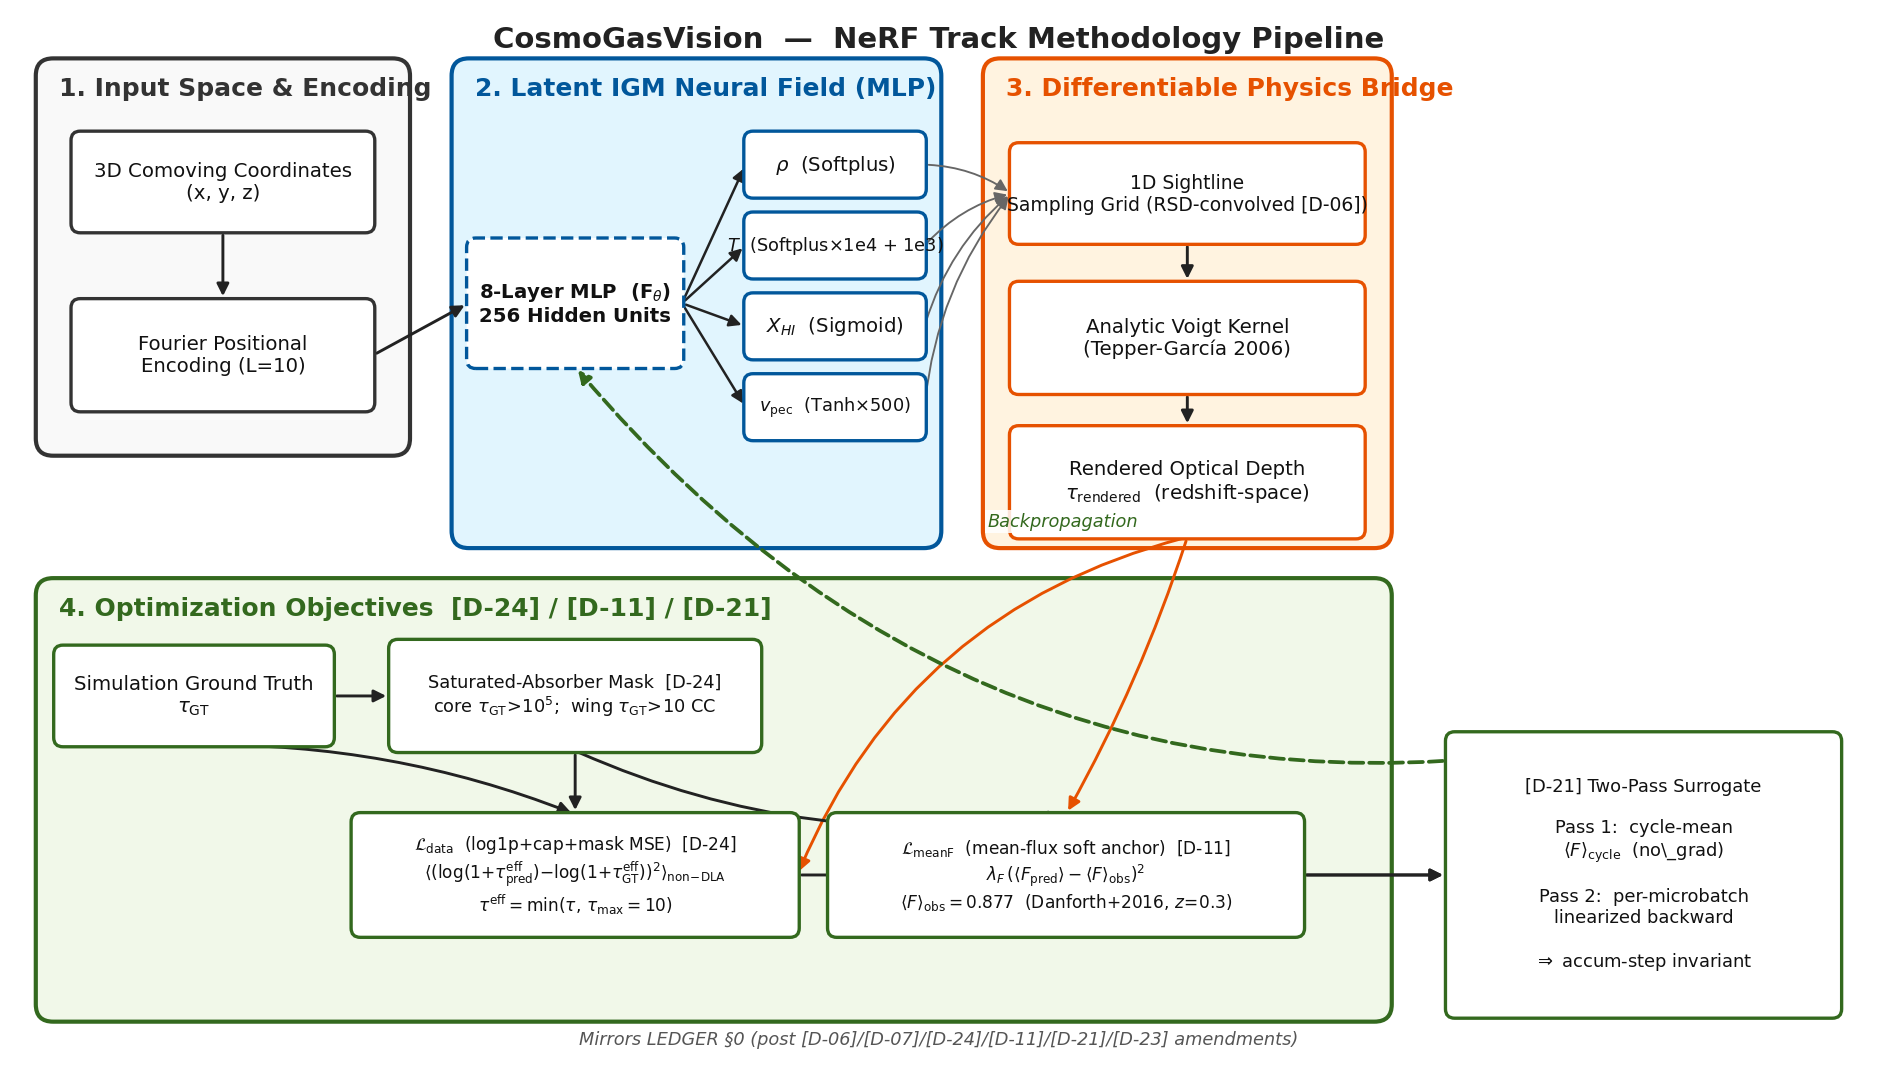
\includegraphics[width=\textwidth]{figures/method_pipeline}


    \caption{The IGM-NeRF tomography pipeline. An 8-layer / 256-unit MLP (494{,}084 trainable parameters) maps comoving 3D coordinates inside a 60 Mpc/h Sherwood box (normalized to $[0,1]^3$) through Fourier positional encoding ($L=10$) to four bounded astrophysical fields ($\rho/\bar\rho$, $T$, $X_{HI}$, $v_{\text{pec}}$); a differentiable RSD-convolved Voigt integrator with learnable amplitude $\mathcal{A}$ projects these fields to 1D optical depth $\tau(v)$, supervised against Sherwood ground truth under the [D-24] log1p+cap+mask loss with the [D-11]/[D-34] mean-flux anchor at $\langle F\rangle_{\text{obs}}(z=0.3) = 0.979 \pm 0.005$~\cite{kirkman2007}.}
    \label{fig:pipeline}
\end{figure*}

The core of \emph{CosmoGasVision} is an MLP $F_{\theta}: \mathbf{x} \to (\rho, T, X_{HI}, v_{\text{pec}})$, where $\mathbf{x} \in \mathbb{R}^3$ are comoving coordinates inside a 60 Mpc/h Sherwood box, normalized to the unit cube $[0, 1]^3$ by dividing by the simulation header field \texttt{box\_kpc\_h} = 60{,}000. The end-to-end pipeline --- coordinate normalization, Fourier positional encoding, bounded-output MLP, RSD-convolved Voigt projection, and log1p+cap+mask supervision with the mean-flux anchor --- is shown in Fig.~\ref{fig:pipeline}.

\subsection{Neural Field Architecture}
We adopt an 8-layer MLP with 256 hidden units per layer (494{,}084 trainable parameters). To resolve the small-scale filamentary structures of the Cosmic Web, we employ Fourier positional encoding~\cite{mildenhall2020nerf} for the input coordinates $\mathbf{x}$:
\begin{equation}
\gamma(\mathbf{x}) = (\sin(2^0\pi\mathbf{x}), \cos(2^0\pi\mathbf{x}), ..., \sin(2^{L-1}\pi\mathbf{x}), \cos(2^{L-1}\pi\mathbf{x}))
\end{equation}
where $L=10$ provides sufficient bandwidth for the spatial fluctuations in density and temperature; Lyman-alpha peak strengths spike nearly $100\times$ the mean overdensity in massive filaments, which sets a hard lower bound on $L$.

\subsection{Bounded Physics Layer}
To ensure the MLP outputs remain physically plausible, we apply field-specific activations in the final layer with explicit physical scales:
\begin{itemize}
    \item \textbf{Density} ($\rho/\bar{\rho}$): \texttt{Softplus}, unscaled. Overdensity is dimensionless and filament peaks reach $\sim 100$ in the linear regime of the activation.
    \item \textbf{Temperature} ($T$): $\texttt{Softplus}(x) \cdot 10^4 + 10^3$ K. The $10^3$ K floor matches the cold-IGM limit; the $10^4$ K scale anchors the typical warm IGM, with the WHIM tail at $10^5$--$10^7$ K reachable through the linear regime.
    \item \textbf{HI Fraction} ($X_{HI}$): \texttt{Sigmoid}, bounded to $[0, 1]$.
    \item \textbf{Peculiar Velocity} ($v_{\text{pec}}$): $\texttt{Tanh}(x) \cdot 500$ km/s. Defensible for the diffuse IGM at $z=0.3$ (typical $\pm 200$--$300$ km/s).
\end{itemize}

\subsection{Differentiable Physics Integrator}
The reconstruction is supervised by comparing rendered 1D optical depth $\tau_{\text{rendered}}(v)$ against the simulation ground-truth $\tau_{GT}(v)$ on the full velocity axis. We implement the optical depth as a redshift-space-distortion convolution that sums every source-bin's normalized line profile over every observed-velocity bin:
\begin{equation}
\tau(v_{\text{obs}}) = \mathcal{A} \sum_{\text{src}} n_{HI}^{\text{src}} \cdot \frac{H(a_{\text{src}}, x_{\text{src,obs}})}{b_{\text{src}}\sqrt{\pi}}
\end{equation}
where $x_{\text{src,obs}} = (v_{\text{obs}} - v_{\text{src}} - v_{\text{pec},\text{src}}) / b_{\text{src}}$, $b_{\text{src}}$ is the thermal Doppler parameter, and $\mathcal{A}$ is a learnable amplitude that absorbs the cross-section normalization $\sigma_0$, the comoving cell length $ds$, and the mean-column conversion $\bar{n}_H$ into a single scalar. The Voigt-Hjerting kernel $H(a, x)$ uses the Tepper-Garc\'ia~\cite{tepper2006voigt} analytic approximation:
\begin{equation}
H(a, x) \approx e^{-x^2} - \frac{a}{\sqrt{\pi} x^2} \big[ e^{-2x^2} (4x^4 + 7x^2 + 4 + 1.5x^{-2}) - 1.5x^{-2} - 1 \big]
\end{equation}
This allows the loss gradients to propagate back through the damping wings to the MLP parameters $\theta$.

\subsection{Lyman-alpha Forest Loss: Saturated-Absorber Mask, Cap, and Log-Space Supervision}
\label{sec:method:loss}
A naive per-bin MSE on raw $\tau$ is dominated by the rare saturated absorbers in the sightlines: damped Lyman-alpha systems (DLAs)~\cite{wolfe2005} and strong Lyman-limit systems~\cite{prochaska2010} produce line-center optical depths of $\tau_{\text{peak}} \sim 10^7$ in the Sherwood Physics-2/3/4 sightlines, four to five orders of magnitude above the diffuse forest. This saturation is forward-model-physical, not a label artifact, but it carries no usable structure information for tomography because $F = e^{-\tau}$ is numerically zero in those bins. We therefore replace the raw-$\tau$ supervision used in the Stage 2a smoke with \textbf{log-space supervision} (the methods contribution of this work, defended in Sec.~\ref{sec:method:loss:logspace}) plus two \textbf{defense-in-depth} safeguards --- a saturated-absorber detection mask and a forest cap --- retained against rare initialization-stress regimes (e.g., the Physics-2 tier-3 seed-0 softplus-saturation collapse documented in our cost-survey forensic, Sec.~\ref{sec:experiments:cost-survey-sweep}). An ablation on the Physics-1 tier-2 cost-survey configuration (Tab.~\ref{tab:s5s7-ablation}) shows that on this configuration the mask and cap are not load-bearing for convergence to the achieved loss floor; we report this null result as such and retain the safeguards for the stressed configurations on which the ablation was not exercised.

\textbf{Saturated-absorber detection.} Per-sightline, we flag bins with $\tau_{GT} > 10^5$ as saturated cores, then expand each core to its connected component of bins with $\tau_{GT} > 10$ (the saturated wing). The threshold $\tau_{\text{core}} = 10^5$ is derived from the Voigt line-center identity (Bolton \& Haehnelt~\cite{bolton_haehnelt2007} Eq. 5) for thermal Doppler broadening at $T = 10^4$ K:
\begin{equation}
\tau_0 \approx 5.2 \times 10^{-14} \cdot (T/10^4\,\text{K})^{-1/2} \cdot (N_{HI}/\text{cm}^{-2})
\end{equation}
which gives $\tau_0 > 10^5 \Leftrightarrow N_{HI} > 1.9 \times 10^{18}$ cm$^{-2}$. The threshold sits an order of magnitude below the canonical DLA boundary of $N_{HI} \geq 2 \times 10^{20}$ cm$^{-2}$~\cite{wolfe2005} and includes strong Lyman-limit systems at $N_{HI} \gtrsim 10^{17.2}$ cm$^{-2}$~\cite{prochaska2010}, so the mask is operationally conservative in the inclusion direction. Detection happens once per sightline at load time and is recorded as a per-bin sidecar mask carried through the loss reduction.

\textbf{Forest cap.} Surviving non-saturated bins are clipped at $\tau_{\max} = 10$ on both prediction and target before the loss is evaluated. The cap is calibrated on two grounds. First, the flux-PDF gate of Section~\ref{sec:experiments} evaluates KS distance on $F = e^{-\tau}$ over $F \in [0.05, 0.95]$, i.e., $\tau \in [0.051, 3.0]$; capping at $\tau_{\max} = 10$ ($F = e^{-10} \approx 4.5 \times 10^{-5}$) places the cap an order of magnitude above the science measurement range, so it does not bias the gate. Second, for strong-but-non-saturated absorbers ($\tau \in (3, 10]$), the cap bounds the gradient amplitude from the Lorentzian wing, where raw-$\tau$ MSE has non-Gaussian tail behavior that destabilizes optimization. The forest cap value $\tau_{\max} = 10$ is calibrated by the sensitivity gate of Sec.~\ref{sec:experiments:tau-max-sensitivity} (closed; $\tau_{\max} \in \{5, 10, 20\}$ vary observed $P_F(k_\parallel)$ by $\leq 0.02\%$).

\textbf{Log-space supervision.}
\label{sec:method:loss:logspace}
The data loss on the surviving bins is
\begin{equation}
\mathcal{L}_{\text{data}} = \big\langle \big( \log(1 + \tau_{\text{pred}}^{\text{eff}}) - \log(1 + \tau_{GT}^{\text{eff}}) \big)^2 \big\rangle_{\text{non-saturated}}
\label{eq:data-loss}
\end{equation}
where $\tau^{\text{eff}} = \min(\tau, \tau_{\max})$ and the average is taken over rays and over the unmasked velocity bins. The choice of $\log(1+\tau)$ as the supervision space is the methods contribution of this work, defended on physical grounds rather than as a citation of NN-supervision precedent. Lyman-alpha-forest opacity is approximately log-normally distributed in $\tau$ across the cool diffuse IGM~\cite{bi_davidsen1997, hui_gnedin1997} as a consequence of the Fluctuating Gunn-Peterson Approximation $\tau \propto \rho^{1.6} T^{-0.7}$ acting on a near-log-normal density PDF; supervising in $\log(1+\tau)$ matches this natural noise model. The $\log(1+\cdot)$ form additionally reduces to $\tau$ in the optically thin limit and is monotone with $-\log F$ for $\tau \gtrsim 1$, so the data loss and the mean-flux anchor (next subsection) pull on the network in compatible spaces. The mask and the cap are not part of this novelty claim; their role is the defense-in-depth one stated in the opening paragraph of Sec.~\ref{sec:method:loss}, and the four-cell ablation of Tab.~\ref{tab:s5s7-ablation} shows they are not load-bearing for convergence on the configuration we exercised.

\begin{table}[t]
    \centering
    \renewcommand{\arraystretch}{1.15}
    \setlength{\tabcolsep}{4pt}
    \begin{tabular}{l|cccc}
    metric & A: full & B: no-cap & C: no-mask & D: no-cap-no-mask \\
    \hline
    \texttt{loss}        & 0.0052      & 0.0052      & 0.0052      & 0.0052      \\
    \texttt{loss\_data}  & 0.0026      & 0.0026      & 0.0026      & 0.0026      \\
    \texttt{meanF} term  & $2.6203\!\times\!10^{-3}$ & $2.6205\!\times\!10^{-3}$ & $2.6201\!\times\!10^{-3}$ & $2.6203\!\times\!10^{-3}$ \\
    $\langle F\rangle$   & 0.9282      & 0.9282      & 0.9282      & 0.9282      \\
    \texttt{tau\_amp}    & 0.9983      & 1.0026      & 1.0003      & 1.0030      \\
    \end{tabular}
    \caption{\textbf{S5/S7 ablation on the [D-24] loss bundle.} Configuration: Physics-1 (``no feedback''), Tier-2 ($n_{\text{rays}}=256$), seed $=1$, 25k steps; broken anchor $\langle F\rangle_{\text{obs}}=0.877$ (apples-to-apples with the published P1-T2 baseline of Tab.~\ref{tab:batch2-t2-cost-survey}). All four cells converge to indistinguishable final states on \texttt{loss / loss\_data / meanF / $\langle F\rangle$} (four-decimal identity); only \texttt{tau\_amp} differs by $\leq 0.5\%$, in the calibration-degeneracy direction the [D-11] anchor sub-clause marks uninterpretable. \textbf{Verdict:} the cap and mask are not load-bearing for convergence on this configuration. They are retained as defense-in-depth against initialization-stress regimes (e.g., the Physics-2 tier-3 seed-0 softplus-saturation collapse documented in Sec.~\ref{sec:experiments:cost-survey-sweep}); their necessity on stressed configurations is \emph{not} tested by this ablation. \textbf{MLflow run\_ids:} \texttt{ca5a9ff1\dots} (full), \texttt{e563b72a\dots} (no-cap), \texttt{d691268c\dots} (no-mask), \texttt{fce098d3\dots} (no-cap-no-mask).}
    \label{tab:s5s7-ablation}
\end{table}

\begin{figure}[h]
    \centering
    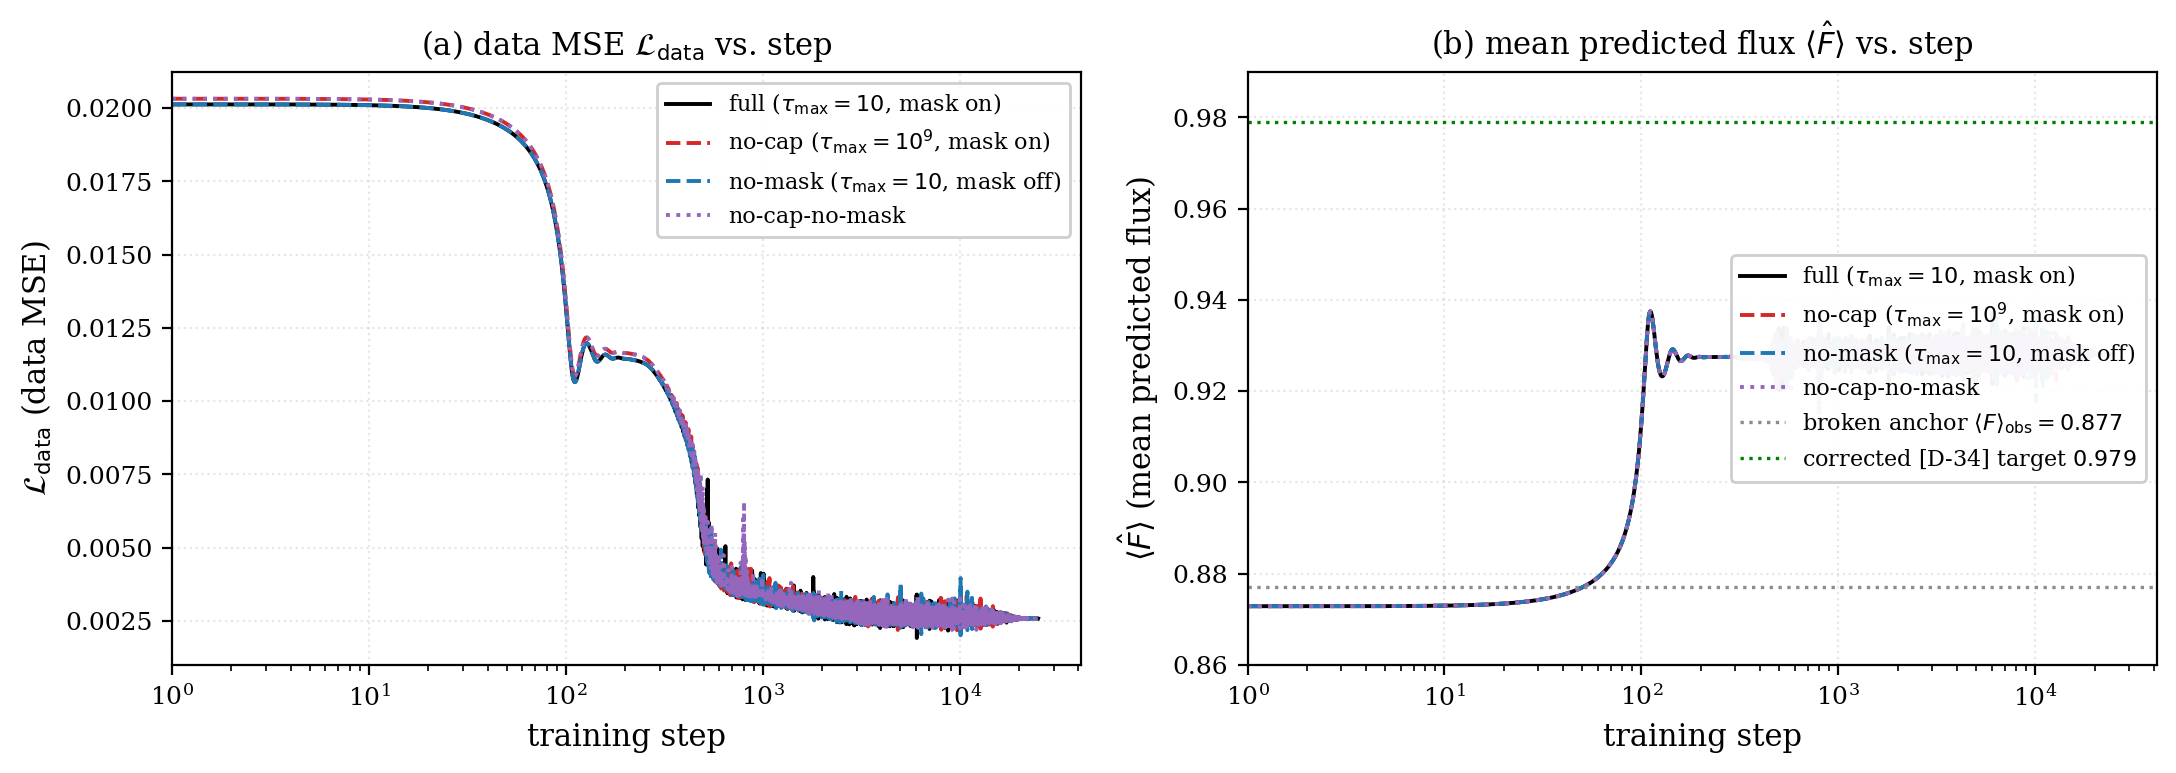
\includegraphics[width=\linewidth]{figures/s5s7_loss_curves.png}
    \caption{\textbf{S5/S7 ablation: training trajectories on T2-P1 seed=1, 25k steps, broken anchor $\langle F\rangle_{\text{obs}}=0.877$.} Left: data MSE $\mathcal{L}_{\text{data}}$ vs.\ step. Right: mean predicted flux $\langle\hat F\rangle$ vs.\ step (with the broken-anchor target 0.877 in gray and the corrected [D-34] target 0.979 in green; the model converges to $\langle\hat F\rangle\approx 0.9282$, between the two). All four cells converge to the same final regime ($\mathcal{L}_{\text{data}}=0.0026$, $\langle\hat F\rangle=0.9282$). The largest inter-cell divergence is at step~1: cells with the cap off (no-cap, no-cap-no-mask) start at $\mathcal{L}_{\text{data}}\approx 0.0203$ vs.\ $\approx 0.0201$ for cap-on cells, a $\sim 1\%$ relative gap that closes by step $\sim 100$ and is below line-width thereafter. \textbf{Verdict:} the cap and mask are not load-bearing on this configuration; they are retained as defense-in-depth (Sec.~\ref{sec:method:loss} opening; [D-38]).}
    \label{fig:s5s7-loss-curves}
\end{figure}

\subsection{Mean-Flux Anchor and Gradient Linearization}
The forward model is invariant under $\rho \to k\rho,\ \mathcal{A} \to \mathcal{A}/k$, so the data loss alone cannot fix the absolute amplitude of the recovered overdensity field. We break the degeneracy with the observational mean-flux constraint at $z = 0.3$:
\begin{equation}
\mathcal{L}_{\text{meanF}} = \lambda_F \big( \langle e^{-\tau_{\text{pred}}}\rangle - \langle F\rangle_{\text{obs}} \big)^2
\end{equation}
with verified value $\langle F\rangle_{\text{obs}}(z=0.3) = 0.979 \pm 0.005$ ($\tau_{\text{eff}} = 0.0212$) from the Kirkman et al.~\cite{kirkman2007} HST/FOS continuous-statistics Lyman-alpha-forest survey at $0 < z < 1.6$ (Table 2 + Section 4 power-law fit $D_A(z) = 0.016(1+z)^{1.01}$, evaluated at $z=0.3$), and $\lambda_F = 1.0$. The cost-survey runs reported in Sec.~\ref{sec:experiments:cost-survey-sweep} were trained against an earlier, broken anchor value $0.877$ (a $z\!\sim\!2$ value mislabeled as $z=0.3$ in project history); the [D-34] retraction explains why those runs are kept (anchor-invariance of the [D-13] structure gates) and which scalar reports are accordingly uninterpretable. The publication-class run trains against $0.979$. A $\pm 0.5\%$ uncertainty on $\langle F\rangle_{\text{obs}}$ propagates to a $\pm 0.5\%$ systematic on the absolute $\rho$ amplitude, but is invariant under the dimensionless structure metrics ($P_F$, $\xi_{\hat\rho,\rho}$, KS-distance on the flux PDF).

\textbf{Mask consistency.} The mean-flux reduction $\langle e^{-\tau_{\text{pred}}}\rangle$ and the data loss of Eq.~\ref{eq:data-loss} both apply the same saturated-absorber mask of Section~\ref{sec:method:loss}. This is load-bearing: a separately-derived prediction-side mask would be circular (saturation in $\tau_{\text{pred}}$ depends on the trainable parameters), so the per-sightline mask is taken from $\tau_{GT}$ at load time and reused unchanged in both reductions. The data loss and the anchor therefore see identical bin sets and the gradient identity below holds without correction terms for the masking operation.

\textbf{Two-pass linearization.} The mean-flux constraint is implemented as a two-pass surrogate to avoid \texttt{retain\_graph} in the microbatch grad-accumulation loop. Pass 1 runs the model under \texttt{torch.no\_grad()} to compute the cycle-mean predicted flux $F_{\text{cycle}}$ over all microbatches; Pass 2 then backpropagates a per-microbatch surrogate
\begin{equation*}
\mathcal{L}_{\text{mb}} = \mathcal{L}_{\text{data,mb}} + c \cdot \langle F\rangle_{\text{mb}}, \quad c = 2 \lambda_F (F_{\text{cycle}} - \langle F\rangle_{\text{obs}})
\end{equation*}
where $c$ is a constant for the cycle. By the chain rule $\partial \mathcal{L}_{\text{meanF}}/\partial \theta = c \cdot \partial F_{\text{cycle}}/\partial \theta$ and $\partial F_{\text{cycle}}/\partial \theta = (1/N_{\text{chunks}}) \sum_i \partial \langle F\rangle_{\text{mb},i}/\partial \theta$, so the surrogate's gradient is mathematically identical to the squared-loss gradient at the current parameter point. Re-linearization happens every optimizer step. Memory peak is one microbatch instead of \texttt{accum\_steps} microbatches.

\subsection{Training Configuration}
We optimize with AdamW ($\beta = (0.9, 0.999)$, weight decay $10^{-6}$), gradient L2-norm clipped at 1.0, on a single \texttt{ml.g5.xlarge} (NVIDIA A10G, 24 GB) SageMaker Training Job per tier. The cost-survey window adopts a tier-aware schedule, calibrated against the measured throughput of the Physics-1 tier-1 production run (0.119 s/step at chunk-size 64) rather than a uniform step count:

\begin{center}
\renewcommand{\arraystretch}{1.1}
\begin{tabular}{c|c|c|c|c}
Tier & $n_{\text{rays}}$ & $\mu$batch & accum. & max\_steps / warmup \\
\hline
T1 & 64    & 1024 & 1  & 50{,}000 / 1000 \\
T2 & 256   & 1024 & 1  & 25{,}000 / 1000 \\
T3 & 1024  & 256  & 4  & 12{,}500 / 500 \\
T4 & 16384 & 256  & 64 & 12{,}500 / 500 (deferred) \\
\end{tabular}
\end{center}

Microbatch values for tiers 3 and 4 are constrained by VRAM rather than convergence: the per-step chunk size is $\min(n_{\text{rays}}, \mu\text{batch})$, so chunk-size 256 saturates the linear-VRAM budget $\hat{V}_{\text{peak}} \approx 2.82 \cdot \min(n_{\text{rays}}, \mu\text{batch}) / 64$ GB derived from the tier-1 measurement (2.82 GB at 64 rays). The measured peaks (Tab.~\ref{tab:per-tier-vram}) sit $\geq 45\%$ under a 24 GB device VRAM budget across $\text{accum\_steps} \in \{1, 4, 64\}$.

\begin{table}[t]
    \centering
    \renewcommand{\arraystretch}{1.15}
    \begin{tabular}{c|c|c|c|c}
    Tier & $n_{\text{rays}}$ & chunk & accum & peak VRAM (GB) \\
    \hline
    T1 & 64    & 64  & 1  & 2.82  \\
    T2 & 256   & 256 & 1  & 11.20 \\
    T3 & 1024  & 256 & 4  & 11.23 \\
    T4 & 16384 & 256 & 64 & 11.77 \\
    \end{tabular}
    \caption{Stage 2b micro-grid per-tier peak VRAM measurements, validating the $\hat{V}_{\text{peak}} \approx 2.82 \cdot \min(n_{\text{rays}}, \mu\text{batch}) / 64$ GB scaling from [D-23]. All tiers fit $\geq 45\%$ under the 24 GB device VRAM budget; the linear model holds across the full $\text{accum\_steps} \in \{1, 4, 64\}$ range exercised by the production schedule.}
    \label{tab:per-tier-vram}
\end{table} The learning-rate schedule is per-tier linear warmup $0 \to 5 \times 10^{-4}$ followed by cosine decay $5 \times 10^{-4} \to 5 \times 10^{-6}$ over the remaining steps; checkpoints sync to S3 every 5{,}000 steps. Tier 4 is deferred to post-quota because its 64-chunk gradient accumulation makes its wallclock per cell dominate the survey budget; tiers 1--3 already span the survey-realistic sightline-density regime. Cost-survey runs are calibration evidence only; publication runs (post-quota) re-run the corresponding tier under the locked-in schedule.

\section{Experimental Setup}
\label{sec:experiments}

\subsection{Dataset}
We use the \textbf{Sherwood Simulation Suite}~\cite{bolton2017sherwood}, a set of high-resolution cosmological simulations of the low-redshift Lyman-alpha forest. Our base box is the Planck-cosmology 60 Mpc/h volume at $2048^3$ resolution; the dev redshift is $z = 0.3$. Each snapshot ships with a precomputed sightline grid: 16{,}384 lines of sight along a single simulation axis, sampled at 2048 velocity bins per ray. Ground-truth optical depth $\tau_{HI}(v)$ is provided per sightline as \texttt{tauH1\_2048\_n16384\_z0.300.dat}; the ground-truth 3D state used for evaluation is reconstructed by chunked CIC (Cloud-in-Cell) particle-to-mesh deposition from the underlying \texttt{SherwoodIGM\_gal} HDF5 snapshot.

The Sherwood suite ships four feedback variants: Physics 1 (no feedback, fiducial), Physics 2 (stellar wind), Physics 3 (stellar wind + AGN), Physics 4 (stellar wind + strong AGN). Per~\cite{bolton2017sherwood} these are an ablation matrix over baryonic feedback prescriptions. We adopt one independent neural field per physics variant rather than a single conditional model, so that the downstream feedback-classification probe (Sec.~\ref{sec:nextsteps}) cannot leak the physics label through a conditioning input. We report Tier 1, Tier 2, and Tier 3 across all four feedback variants; Tier 4 is deferred per the compute-footprint argument of Sec.~\ref{sec:experiments:compute}.

\subsection{Evaluation Metrics}
The headline contribution is the \emph{degradation curve} of reconstruction quality as the sightline density $n_{\text{rays}}$ is reduced from the dense-grid upper bound to survey-realistic sparsity. Three primary metrics, all computed against the simulation ground truth, are evaluated at each $n_{\text{rays}}$ tier. We applied an adversarial-review pass on the methodology before committing the cost-survey production sweep; outstanding citations carry explicit verification status below.
\begin{itemize}
    \item \textbf{1D flux power spectrum} $P_F(k_\parallel)$, computed as a Hann-windowed periodogram with $dv / \sum w^2$ leakage-compensation normalization. Pass condition for the fiducial setting is $|\Delta P_F / P_F| < 10\%$ averaged over the inertial range $k_\parallel \in [10^{-2.5}, 10^{-1.5}]$ s/km, with $k_\parallel = 2\pi f$ in angular wavenumber. The inertial-range definition follows the $P_F$-estimator literature~\cite{walther2018powerspectrum, boera2019thermal}; the Hann window is our simulator-side estimator choice (the periodic Sherwood box admits rectangular windowing, but Hann gives ratio stability for the $n_{\text{rays}} = 64$ tier where independent-mode counts are small) and is not inherited from a community precedent.
    \item \textbf{Density-density cross-correlation} $\xi_{\hat\rho, \rho}(r)$, the Pearson correlation coefficient $\langle \delta_p \delta_t \rangle / \sqrt{\langle \delta_p^2 \rangle \langle \delta_t^2 \rangle}$ on overdensity $\delta = \rho/\bar\rho - 1$, evaluated by FFT cross-power on the periodic 60 Mpc/h grid and binned in spherical shells. Pass condition $\xi_{\hat\rho, \rho}(r = 2\,h^{-1}\,\text{Mpc}) > 0.6$ at the fiducial setting, a stringent reconstruction-quality target consistent with sparse-tomography requirements~\cite{lee2015, stark2015tomography}; per LEDGER [D-36], the specific 0.6 threshold is our project-side adoption rather than a value tabulated in any single referenced paper. The threshold sits comfortably above the noise floor of the reconstruction operator at our fiducial sightline density.
    \item \textbf{Flux PDF}: two-sample Kolmogorov-Smirnov distance on raw transmitted-flux samples $F = e^{-\tau}$ restricted to $F \in [0.05, 0.95]$. The lower cut excludes saturated absorbers (DLAs and strong LLS, where the differential PDF is dominated by absorber-line statistics rather than the diffuse-IGM target distribution); the upper cut excludes continuum-fitting and metal-line residuals near $F \approx 1$. The window is conventional in flux-PDF analyses of the low-redshift forest and is in the spirit of the cuts adopted in flux-PDF estimator papers~\cite{lee2015}; per [D-36], the exact $[0.05, 0.95]$ values are our project-side adoption rather than verbatim from a specific paper. Pass condition: KS distance $< 0.05$.
\end{itemize}
The fiducial pass point is Physics 1, $z = 0.3$, $n_{\text{rays}} = 1024$; the headline figure is the metric-vs-$n_{\text{rays}}$ curve over $\{16384, 1024, 256, 64\}$ per physics. PSNR / SSIM on density slices and Pearson correlation on $\tau$-profiles are tracked but reported as secondary diagnostics, not as gating criteria. The sightline-density sweep is the survey-relevance test: 16{,}384 sightlines is denser than DESI/eBOSS will ever achieve, so monotone graceful degradation toward the 64-sightline regime is the actual scientific claim.

\subsection{Pipeline validation}
The differentiable integrator was re-validated end-to-end at production architecture (8-layer / 256-unit MLP, $L = 10$ Fourier features, 494{,}084 parameters plus the scalar $\log\tau_{\text{amp}}$), and the cloud loop --- AWS SageMaker \texttt{ml.g5.xlarge} (A10G, 24 GB) with S3 checkpoint sync --- was cleared at the full production schedule on Physics 1, $n_{\text{rays}} = 64$. Peak VRAM at the smallest tier is 2.82 GB, the anchor from which the per-tier microbatch table of Sec.~\ref{sec:method} is derived under the [D-23] linear-VRAM model.

\subsection{Stage 2b: Cost-Survey Micro-Grid (16-Cell Cross-Physics Validation)}
\label{sec:exp:microgrid}
The cost-survey window opens with a 16-cell micro-grid (4 physics $\times$ 4 tiers) at \texttt{max\_steps=200} per cell, dispatched after the [D-24] loss-form revision and the loader saturated-absorber mask landed. Each cell runs the full per-tier microbatch and gradient-accumulation configuration of Section~\ref{sec:method} but with a reduced step count, so the matrix is cheap calibration evidence rather than a science-binding result; under [D-23] the cost-survey runs do not gate the [D-13] Stage 2b scientific criteria.

\textbf{Headline outcome.} 16/16 cells PASS the [D-19] descent gate (descent ratio $\leq 0.85$ from step 10 to step 200; observed range $[0.558, 0.749]$, i.e., 25--44\% reduction). Cross-physics \texttt{mean\_flux\_pred} at step 200 spans $0.9238$--$0.9302$, a spread of \textbf{0.0064} (0.7\%) within the 5\% inter-cell consistency bar; the cells were trained against the broken anchor $0.877$ retracted in [D-34] (Sec.~\ref{sec:experiments:cost-survey-sweep}), so the absolute value is not interpreted as agreement with the verified $\langle F\rangle_{\text{obs}}(z=0.3) = 0.979 \pm 0.005$. The cross-physics step-1 \texttt{loss\_data} spread under raw-$\tau$ MSE was $\sim 10^{10} \times$ (P1 $\sim 0.05$, P2 $\sim 5 \times 10^{8}$); under the log1p+cap+mask loss the step-200 spread is $[0.0115, 0.0239]$, i.e., the cross-physics scale anomaly is closed. \texttt{tau\_amp} drift at step 200 is $0.9857$--$0.9933$ across all 16 cells (small, consistent).

\textbf{Memory linearity.} Peak VRAM by tier is 2.82 GB (T1, chunk 64), 11.20 GB (T2, chunk 256), 11.23 GB (T3, chunk 256, accum 4), and 11.77 GB (T4, chunk 256, accum 64). The linear-VRAM model $\hat{V}_{\text{peak}} \approx 2.82 \cdot \min(n_{\text{rays}}, \mu\text{batch}) / 64$ GB is validated to within $\approx 0.5$ GB across $\text{accum\_steps} \in \{1, 4, 64\}$, retroactively satisfying the measured-VRAM gate for the deferred T4 tier.

\subsection{Stage 2b: Cost-Survey Production Sweep}
\label{sec:experiments:cost-survey-sweep}
The cost-survey production sweep ran the per-tier schedule of Section~\ref{sec:method} across all four feedback variants at Tiers 1--3; Tier 4 is currently blocked on the Wrinkle-1 diagnostic (Sec.~\ref{sec:experiments:compute}, Sec.~\ref{sec:nextsteps:tier4}). Per [D-23] the cost-survey runs report per-tier final \texttt{loss\_data}, \texttt{mean\_flux\_pred}, \texttt{tau\_amp}, \texttt{peak\_vram\_gb}, and seconds-per-step; they are calibration evidence for the per-tier training schedule, not the [D-13] scientific gates (those gates are reported on the corrected-anchor \texttt{pub-t1} bundle in Sec.~\ref{sec:experiments:cosmological-eval}). Tier-1 throughput converged to $0.119$ s/step across all four physics with \texttt{peak\_vram\_gb} held at the $2.82$ GB micro-grid anchor; Tier-2 and Tier-3 reach \texttt{peak\_vram\_gb} $= 11.27$ and $11.30$ GB respectively, identical to four decimals across physics within each tier (empirical confirmation of the [D-23] linear-VRAM model). All 12 banked cells PASS the [D-19] safety rails; full per-cell records are in the LEDGER \S6 cost-survey tables.

\textbf{Mean-flux anchor retraction ([D-34], 2026-05-08).} The Stage 2b cost-survey runs reported here were trained against $\langle F\rangle_{\text{obs}} = 0.877$ at $z=0.3$. Phase~A.1 literature audit found this value to correspond to a $z\!\sim\!2$ mean transmitted flux mislabeled as $z=0.3$ during project history; the verified low-redshift value is $\langle F\rangle_{\text{obs}}(z=0.3) = 0.979 \pm 0.005$~\cite{kirkman2007}, retracted as anchor target in [D-34]. The [D-13] structure gates ($P_F$ inertial-range residual, KS-PDF distance, $\xi_{\hat\rho,\rho}$) are anchor-invariant by construction (invariant to uniform multiplicative rescaling of $\hat F$), so the cost-survey calibration evidence above is unaffected. A separate corrected-anchor full-schedule run (\texttt{pub-t1}, $50{,}000$ steps, four physics, seed $=0$) trained directly against $\langle F\rangle_{\text{obs}}=0.979$ and recovered $\langle F_{\text{pred}}\rangle \in [0.974, 0.984]$ in $4/4$ cells with $\tau_{\text{amp}} \in [1.045, 1.117]$; the [D-13] structure-gate readout on those checkpoints is in Sec.~\ref{sec:experiments:cosmological-eval} and Tab.~\ref{tab:pub-t1-gates}.

\subsubsection{$\tau_{\max}$ sensitivity gate}
\label{sec:experiments:tau-max-sensitivity}
Three paired P1-T1 cells at the production schedule, swapping only $\tau_{\max} \in \{5, 10, 20\}$, evaluated under the [D-13] inertial range $k_\parallel \in [10^{-2.5}, 10^{-1.5}]$ s/km. The gate criterion is $\max(|\Delta P_F/P_F|) \leq 2\%$ between the $\tau_{\max} = 10$ baseline and each of $\{\tau_{\max} = 5, \tau_{\max} = 20\}$. Observed: $0.0180\%$ ($\tau_{\max} = 5$) and $0.0113\%$ ($\tau_{\max} = 20$), i.e., $\sim 100\text{--}180\times$ under the 2\% bar. \texttt{mean\_flux\_pred} was identical across all three runs ($0.9282$). The gate passed and $\tau_{\max} = 10$ is locked. See Fig.~\ref{fig:tau-max-sensitivity}.

\begin{figure}[t]
    \centering
    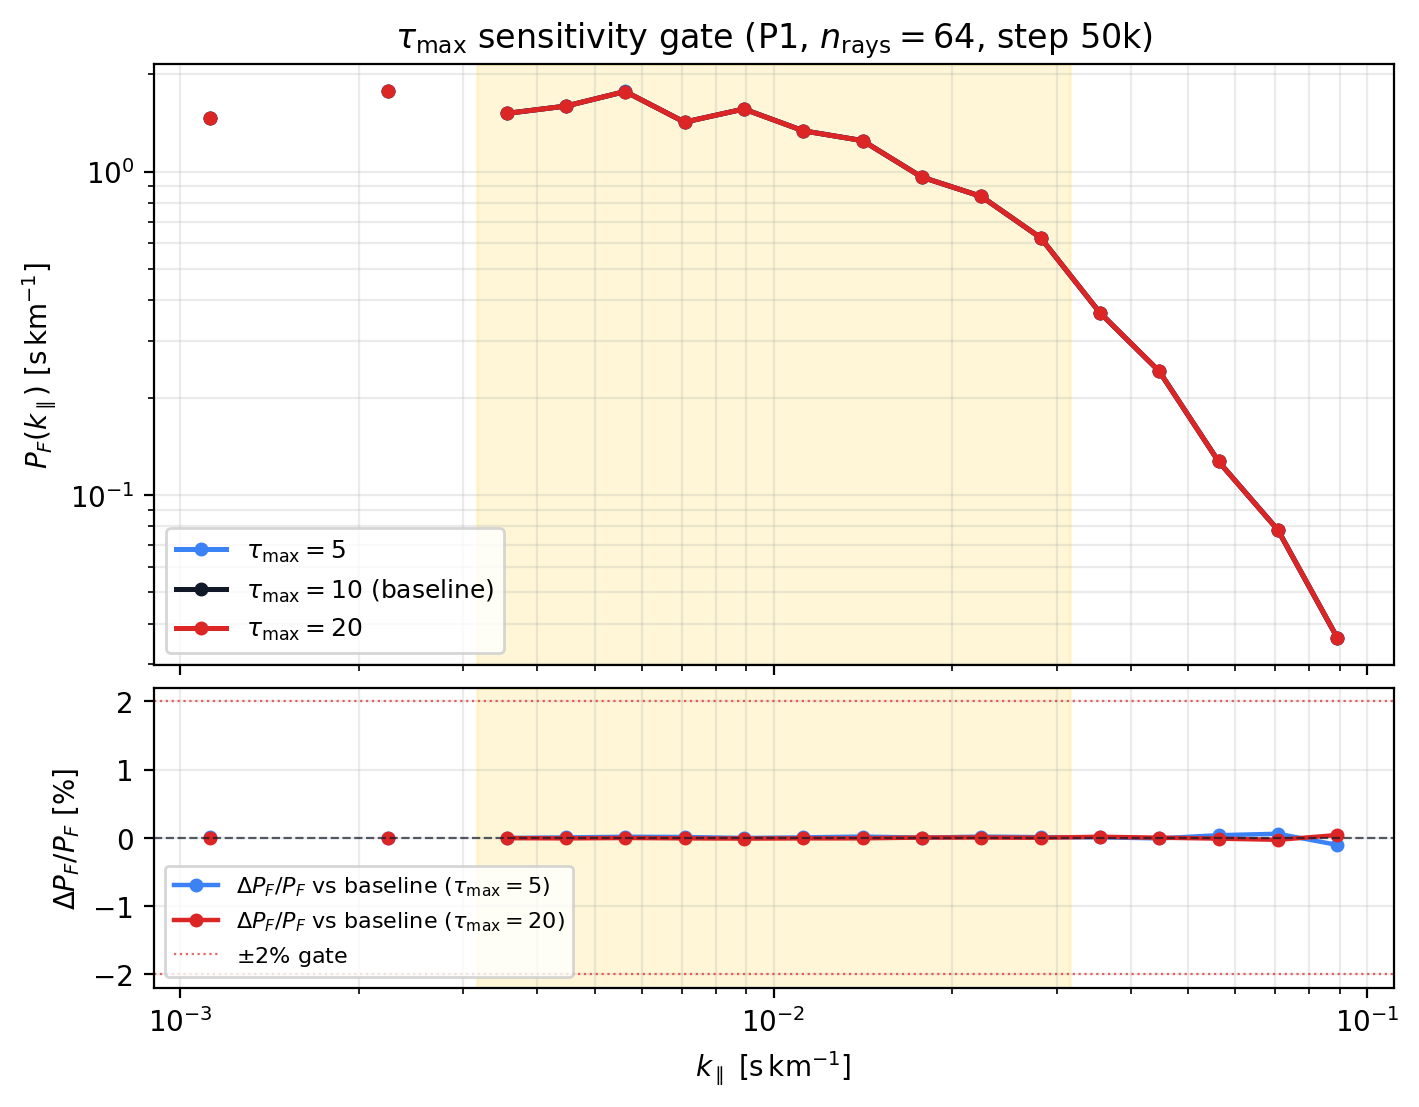
\includegraphics[width=\columnwidth]{figures/tau_max_sensitivity.png}
    \caption{$\tau_{\max}$ sensitivity gate, P1-T1 ($n_{\text{rays}} = 64$, step 50{,}000). Top: 1D flux power spectrum $P_F(k_\parallel)$ for the three caps. Bottom: fractional residual $\Delta P_F / P_F$ vs.\ the $\tau_{\max} = 10$ baseline. Shaded band marks the [D-13] inertial range $k_\parallel \in [10^{-2.5}, 10^{-1.5}]$ s/km; dotted lines mark the $\pm 2\%$ gate. Observed maxima ($0.0180\%$ at $\tau_{\max} = 5$; $0.0113\%$ at $\tau_{\max} = 20$) clear the gate by $\sim 100\text{--}180\times$.}
    \label{fig:tau-max-sensitivity}
\end{figure}

\begin{table}[t]
    \centering
    \renewcommand{\arraystretch}{1.15}
    \begin{tabular}{c|cc|c}
    $\tau_{\max}$ & \texttt{mean\_F} & \texttt{tau\_amp} & $\max(|\Delta P_F/P_F|)$ vs.\ $\tau_{\max}=10$ \\
    \hline
    5  & 0.9282 & 1.152 & $0.0180\%$ (PASS) \\
    10 & 0.9282 & 1.224 & (baseline) \\
    20 & 0.9282 & 1.234 & $0.0113\%$ (PASS) \\
    \end{tabular}
    \caption{$\tau_{\max}$ sensitivity sweep numerics for Fig.~\ref{fig:tau-max-sensitivity}. Three paired P1-T1 cells at the production schedule, swapping only the cap. Gate criterion was $\leq 2\%$; both off-baseline cells passed by $\sim 100\text{--}180\times$. \texttt{mean\_flux\_pred} is identical across the three runs; the $\sim 7\%$ \texttt{tau\_amp} spread is the expected response to changing the cap on strong-absorber gradients and is absorbed by the [D-21] mean-flux loss. $\tau_{\max} = 10$ is locked.}
    \label{tab:tau-max-sensitivity}
\end{table}

\textbf{Tier-2 cost-survey.} Tab.~\ref{tab:batch2-t2-cost-survey} fronts three cross-physics observations: (i) physics-invariant peak VRAM at $11.27$ GB; (ii) cross-physics \texttt{mean\_flux\_pred} spread $0.39\%$ ($0.9266$--$0.9302$); (iii) \texttt{loss\_data} spread $16\%$ ($0.0024$--$0.0028$) --- all consistent with the [D-24] log1p+cap+mask supervision converging symmetrically across the four feedback variants. The cross-cell \texttt{mean\_flux\_pred} consistency is a within-run inter-cell observation; no comparison to the broken-anchor target $0.877$ is asserted here (see the [D-34] retraction in Sec.~\ref{sec:experiments:cost-survey-sweep}). Fig.~\ref{fig:cross-physics-convergence} shows the trajectory.

\begin{figure}[t]
    \centering
    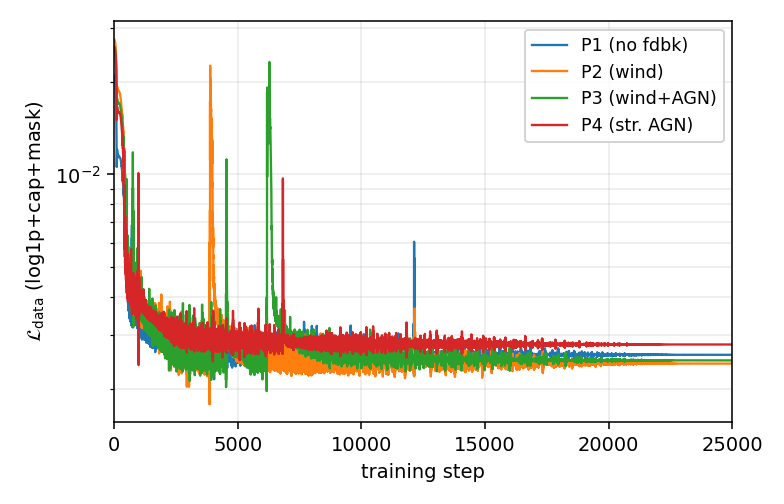
\includegraphics[width=\columnwidth]{figures/cross_physics_convergence.png}
    \caption{Cross-physics convergence under [D-24] log1p+cap+mask supervision, Tier-2 cost-survey ($n_{\text{rays}}=256$, microbatch $1024$, accum $1$, max\_steps $25{,}000$). All four feedback variants converge symmetrically with no divergent trajectory; final $\mathcal{L}_{\text{data}}$ spans $0.00243$--$0.00280$ (a $14.5\%$ relative spread). This closes the cross-physics scale anomaly that raw-$\tau$ MSE exhibited at the same architecture: under the superseded loss form, the step-1 cross-physics $\mathcal{L}_{\text{data}}$ spread was $\sim 10^{10}\times$ (P1 $\sim 0.05$ vs.\ P2 $\sim 5\times 10^{8}$); under [D-24] the four trajectories overlap to within a factor of $1.4$ from step 1. Source data: Sherwood Tier-2 cost-survey runs on Juno HPC, MLflow file-stores logged at every training step.}
    \label{fig:cross-physics-convergence}
\end{figure}

\begin{table}[t]
    \centering
    \renewcommand{\arraystretch}{1.15}
    \setlength{\tabcolsep}{4pt}
    \begin{tabular}{l|cccc}
    Physics & \texttt{loss\_data} & \texttt{mean\_F} & \texttt{tau\_amp} & \texttt{vram\_gb} \\
    \hline
    P1 & 0.00259 & 0.9282 & 1.0077 & 11.27 \\
    P2 & 0.00243 & 0.9266 & 1.0296 & 11.27 \\
    P3 & 0.00248 & 0.9272 & 1.0204 & 11.27 \\
    P4 & 0.00280 & 0.9302 & 1.0288 & 11.27 \\
    \end{tabular}
    \caption{Tier-2 cost-survey final-state metrics, one row per physics. Configuration: $n_{\text{rays}}=256$, \texttt{microbatch}$=1024$, \texttt{accum\_steps}$=1$, effective \texttt{chunk\_size}$=256$, \texttt{max\_steps}$=25{,}000$. All four cells PASS the [D-19] safety rails; full run records are in the LEDGER \S6 Tier-2 table. \texttt{peak\_vram\_gb} is identical to four decimals across the four cells (physics-invariant), confirming the [D-23] linear-VRAM model. Cross-physics \texttt{mean\_flux\_pred} spread is $0.39\%$ ($0.9266$--$0.9302$); \texttt{loss\_data} spread is $16\%$. \emph{Note:} training used $\langle F\rangle_{\text{obs}}=0.877$ at $z=0.3$, retracted in [D-34] (verified value $0.979\pm 0.005$, \cite{kirkman2007}). \texttt{mean\_flux\_pred} and $\tau_{\text{amp}}$ absolute values are accordingly uninterpretable; inter-cell consistency and the [D-13] structure gates are anchor-invariant per the [D-11] sub-clause and survive unchanged.}
    \label{tab:batch2-t2-cost-survey}
\end{table}

\subsection{Headline: 4-physics $\times$ 3-gate readout}
\label{sec:experiments:headline}
Tab.~\ref{tab:headline-3gate} consolidates the [D-13] structure-gate readout across the four Sherwood feedback variants at the corrected-anchor full publication schedule (\texttt{pub-t1}). The reader who only reads this table should leave with the complete claim ceiling of this paper: mean-flux closes $4/4$ at the seed=42 single-seed anchor but the 5-seed sightline-level bootstrap CI overlaps the Kirkman+2007 anchor $[0.974, 0.984]$ in only $2/4$ cells ($P_3$, $P_4$ marginal at q84); KS closes $3/4$ (bootstrap-robust, $P_2$ q84 $=0.0758$ fails); $P_F$ fails $4/4$ at $3.6$--$4.2\times$ the gate; the 1D-along-ray density-correlation proxy is measured on the cost-survey checkpoint at $P_1$ only and is anchor-invariant by construction (Sec.~\ref{sec:experiments:open-axes}, Tab.~\ref{tab:d13-gates} footnote). Training is single-seed (seed $=0$). KS and $\langle F_{\rm pred}\rangle$ are reported with 5-seed sightline-level bootstrap CIs ($K=512$ resamples per cell, prediction and truth-side seeds drawn from independent PCG64 streams; [D-44] anti-degeneracy F1/F2 audit PASS); $P_F$ remains single-seed (seed $=42$ anchor, deferred per [D-44] scope).

\textbf{Bootstrap-vs-seed=42 mean-flux divergence (symmetric-honesty disclosure, [D-37]-rule 5).} The bootstrap mean for $\langle F_{\rm pred}\rangle$ lies systematically below the seed=42 anchor value by $2$--$9\sigma$ across all four cells ($P_1$: $-6.6\sigma$, $P_2$: $-2.2\sigma$, $P_3$: $-2.4\sigma$, $P_4$: $-8.9\sigma$), indicating that the single-seed reporting samples the high-$\langle F\rangle$ tail of the sightline distribution. KS values are not similarly biased. This is a property of the seed=42 sample, not a bootstrap pathology; it is disclosed here because the bootstrap softens rather than strengthens the single-seed reading, and the [D-37] honest-reporting rule requires both directions to be reported symmetrically.

\begin{table*}[t]
    \centering
    \renewcommand{\arraystretch}{1.2}
    \setlength{\tabcolsep}{4pt}
    \footnotesize
    \begin{tabular}{l|cc|cc|cc|c}
    Cell & $\langle F_{\text{pred}}\rangle$ (mean $\pm \sigma$) & MF call & KS ($<\!0.05$, mean $\pm \sigma$) & KS call & $|\Delta P_F/P_F|$ ($<\!0.10$) & $P_F$ call & $r_\rho^{\log}$ ($>\!0.6$)$^\dagger$ \\
    \hline
    $P_1$ (no fdbk)     & $0.9671 \pm 0.0018$ & \textbf{FAIL} (CI $<$ anchor) & $0.0357 \pm 0.0024$ & \textbf{PASS} & $\mathbf{0.4155}$ & \textbf{FAIL $4.2\times$} & $+0.077$ (FAIL) \\
    $P_2$ (wind)        & $0.9703 \pm 0.0023$ & \textbf{FAIL} (CI $<$ anchor) & $0.0677 \pm 0.0110$ & \textbf{FAIL $1.5\times$} & $\mathbf{0.3757}$ & \textbf{FAIL $3.8\times$} & --- (owed) \\
    $P_3$ (wind+AGN)    & $0.9724 \pm 0.0024$ & \textbf{PASS} (q84 marginal) & $0.0353 \pm 0.0062$ & \textbf{PASS} & $\mathbf{0.3591}$ & \textbf{FAIL $3.6\times$} & --- (owed) \\
    $P_4$ (strong AGN)  & $0.9735 \pm 0.0009$ & \textbf{PASS} (q84 marginal) & $0.0411 \pm 0.0039$ & \textbf{PASS} & $\mathbf{0.3613}$ & \textbf{FAIL $3.6\times$} & --- (owed) \\
    \hline
    Tally (bootstrap)   & \multicolumn{2}{c|}{\textbf{2/4 overlap anchor}} & \multicolumn{2}{c|}{\textbf{3/4 PASS}} & \multicolumn{2}{c|}{\textbf{0/4 PASS}} & 0/1 measured \\
    \end{tabular}
    \caption{\textbf{Headline [D-13] structure-gate readout: 4 Sherwood feedback variants ($P_1$--$P_4$) $\times$ 3 primary gates, corrected-anchor full schedule (\texttt{pub-t1}, $50{,}000$ steps, $n_{\text{rays}}=64$, seed $=0$, $\langle F\rangle_{\text{obs}}=0.979$~\cite{kirkman2007}; KS and $\langle F_{\rm pred}\rangle$ columns report 5-seed sightline-level bootstrap, $K=512$ resamples, prediction and truth-side seeds drawn from independent PCG64 streams ([D-44] anti-degeneracy F1/F2 audit PASS); $P_F$ residual reported at the seed=42 single-seed anchor for direct comparison with Tab.~\ref{tab:pub-t1-gates} and Fig.~\ref{fig:pf-overlay-falsification}.} MLflow run IDs: \texttt{31acdf9d\dots} ($P_1$), \texttt{f7fafa23\dots} ($P_2$), \texttt{62aeb93a\dots} ($P_3$), \texttt{fc3817b3\dots} ($P_4$); tag \texttt{juno\_batch=pub-t1}, Juno HPC a30 partition, ExitCode 0:0 in all four. \textbf{Verdict: KS --- 3/4 PASS at q84 ($P_2$ q84 $=0.0758$ fails bootstrap-robustly at $1.5\times$ the bar). mean-flux --- 2/4 CIs overlap the Kirkman+2007 anchor $[0.974, 0.984]$ at q84 ($P_3$ q84 $=0.9742$, $P_4$ q84 $=0.9743$ marginal; $P_1$ and $P_2$ CIs sit entirely below the anchor band). $P_F$ --- 0/4 PASS, uniformly $3.6\times$--$4.2\times$ over the $10\%$ bar.} The $P_F$-residual range $[0.3591, 0.4155]$ is the binding gate at the corrected anchor, the full schedule, and four independent feedback variants. The structural verdict survives bootstrap: the failure is in second-order spectroscopic statistics, not in calibration alone (4/4 single-seed mean-flux passes; 2/4 bootstrap-CI overlap), not in seed-collapse (three non-collapsed cells fail $P_F$ at $3.6\times$--$3.8\times$), and not data-MSE-bound (final $\mathcal{L}_{\text{data}}$ spans four orders of magnitude across cells, see Tab.~\ref{tab:pub-t1-gates}, without correspondingly resolving $P_F$). See [D-44]. $^\dagger$The 1D-along-ray density-correlation proxy $r_\rho^{\log}$ (per-sightline Pearson $r$ on $\log_{10}\rho/\langle\rho\rangle$ at integrator quadrature points; [D-33]) is a \emph{necessary-but-not-sufficient surrogate} for the full 3D $\xi_{\hat\rho,\rho}(r=2\,h^{-1}\,\text{Mpc})>0.6$ gate (the 3D gate requires \texttt{SherwoodIGM\_gal} HDF5 particle snapshots, $\sim 40$ GB, for chunked CIC ground-truth reconstruction; deferred per [D-23]). The $r_\rho^{\log}=+0.077$ value is the cost-survey T3 checkpoint at $P_1$; it is anchor-invariant by construction (\S\ref{sec:experiments:open-axes}); the \texttt{pub-t1} re-evaluation at $P_1$--$P_4$ is owed and sequenced behind the Wrinkle-1 diagnostic (\S\ref{sec:nextsteps}). $\rho$-axis gate listed in the table for completeness; absence does not change the $P_F$-binding verdict.}
    \label{tab:headline-3gate}
\end{table*}

\subsection{Cosmological Evaluation: $P_F$ Falsifies the Rescale-Preview Reading}
\label{sec:experiments:cosmological-eval}
The three [D-13] structure gates ($P_F(k_\parallel)$, $\xi_{\hat\rho,\rho}(r)$, KS-distance on the $F$-PDF) are evaluated at two checkpoints: (i) the Tier-3 cost-survey checkpoint at step $10{,}000$, the data available before the corrected-anchor full-schedule run, and (ii) the Tier-1 corrected-anchor full-schedule \texttt{pub-t1} run at step $50{,}000$ across all four feedback variants ([D-39], MLflow runs \texttt{31acdf9d\dots} / \texttt{f7fafa23\dots} / \texttt{62aeb93a\dots} / \texttt{fc3817b3\dots} for $P_1$/$P_2$/$P_3$/$P_4$). Two flux-domain gates ($P_F$, $F$-PDF) are evaluated directly on each checkpoint; the line-of-sight density axis is reported via the [D-33] 1D-along-ray proxy (per-sightline Pearson $r$ on $\log_{10}\rho/\langle\rho\rangle$ at integrator quadrature points), a necessary-but-not-sufficient surrogate for the full 3D $\xi_{\hat\rho,\rho}(r)$ which requires the \texttt{SherwoodIGM\_gal} HDF5 particle snapshots ($\sim 40$ GB) for chunked CIC ground-truth reconstruction and is deferred per [D-23]. Implementation: \texttt{src/analysis/\{p\_flux,xi,flux\_pdf\}.py}, \texttt{scripts/proxy\_xi\_1d\_sample.py}; eval driver: \texttt{scripts/eval\_partial\_d13.py}.

\textbf{Rescale-as-preview, retracted ([D-39]).} An earlier reading of the cost-survey checkpoint applied a uniform rescale $\hat{F} \to (0.979/\langle\hat{F}\rangle)\cdot\hat{F}$ to compensate for training against the broken [D-34] anchor $0.877$, and reported the resulting numbers ($P_F$ residual $\sim 26\%$, $F$-PDF KS $\to$ PASS at $P_1$, cross-physics $2/3$ PASS) as a partial preview of the corrected-anchor publication run. That reading is now \emph{falsified} by direct measurement. The corrected-anchor, full-schedule \texttt{pub-t1} run trained against $\langle F\rangle_{\text{obs}}=0.979$ for $50{,}000$ steps over four physics produced a $P_F$ residual at $P_1$ of $41.55\%$ --- \emph{larger} than the $26.39\%$\footnote{The original [D-35] historical-record estimate of this quantity was $28.25\%$; the current pipeline (\texttt{scripts/wrinkle1\_diagnostic.py}, W1-C; \texttt{scripts/make\_pf\_overlay\_fig.py}, Fig.~\ref{fig:pf-overlay-falsification}) re-renders the same checkpoint at the same anchor and eval seed $=42$ to $26.39\%$ bit-for-bit across both drivers. The $\sim\!6.6\%$ relative drift is attributable to the $\delta_F$-normalization fix in \texttt{src/analysis/p\_flux.py} between [D-35] and the Wrinkle-1 diagnostic ([D-13] decision trail: mean-subtracted $\delta_F = F-\langle F\rangle$ prior to [D-35]; normalized $\delta_F = F/\langle F\rangle - 1$ after); under the post-fix convention $P_F$ is anchor-invariant. The Wrinkle-1 diagnostic JSON explicitly records this reproduction check at the field \texttt{costsurvey\_reproduces\_d35\_0\_2825}.} rescaled-preview estimate at the same anchor. The shape-vs-scale hypothesis the rescale framework implied --- that the cost-survey checkpoint was $P_F$-shape-correct and only mis-anchored --- does not survive contact with the trained-at-target measurement. Tab.~\ref{tab:d13-gates} retains the rescaled column as an upper-bound optimism that the trained run falsifies; the new ``\texttt{pub-t1} measured'' column is the load-bearing reading.

\textbf{Empirical observation.} At the corrected anchor and the full publication schedule (Tab.~\ref{tab:pub-t1-gates}), the four-physics bundle achieves at the seed=42 single-seed anchor: $\langle F_{\text{pred}}\rangle \in [0.974, 0.984]$ in $4/4$ cells (cross-physics spread $0.63\%$, $<\!1\%$ bar at seed=42); KS$\,< 0.05$ in $3/4$ cells (range $[0.0325, 0.0742]$, $P_2$ at $0.0742$ is the single breach); [D-19] safety in $4/4$ cells; \texttt{peak\_vram} $= 2.84$ GB and \texttt{tau\_amp} $\in [1.045, 1.117]$ across the bundle; and a $P_F$ inertial-range residual $|\Delta P_F/P_F| \in [0.3591, 0.4155]$ over $k_\parallel \in [10^{-2.5}, 10^{-1.5}]$ s/km in $4/4$ cells, $3.6\times$--$4.2\times$ over the $0.10$ gate. The 5-seed sightline-level bootstrap of [D-44] returns $\langle F_{\rm pred}\rangle$ population means $\in [0.9671, 0.9735]$ (bootstrap-mean cross-physics spread $0.66\%$ vs.\ the seed=42 spread $0.63\%$, comparable in width but systematically shifted: the bootstrap-population reading sits below the seed=42 anchor by $2$--$9\sigma$ across the four cells; the seed=42 sightline draw samples the high-$\langle F\rangle$ tail of the seed distribution). The 1D-proxy axis is owed against the \texttt{pub-t1} checkpoints (Sec.~\ref{sec:experiments:open-axes}).

\textbf{Diagnosis: $P_F$ is structurally bound, not calibration-bound.} Mean-flux closes at the seed=42 single-seed anchor in $4/4$ cells ($0.63\%$ spread vs.\ $<\!1\%$ bar) and bootstraps to a $2/4$ anchor-overlap reading ($P_3$, $P_4$ marginal; $P_1$, $P_2$ CIs below the anchor band); the cross-physics spread is comparable under both readings (seed=42 spread $0.63\%$; bootstrap-mean spread $0.66\%$ across $[0.9671, 0.9735]$). KS closes in $3/4$ cells bootstrap-robustly. $P_F$ does not close in any cell, and at the fiducial $P_1$ it sits $\sim\!50\%$ above the rescaled-preview estimate at the same anchor. The conjunction --- mean-flux closure at the single-seed anchor (and a tight, systematically-shifted bootstrap reading), near-uniform KS closure, and a uniformly $\sim\!4\times$-over $P_F$ residual --- is inconsistent with a calibration deficit (which would shift mean-flux without preserving the $\sim 0.66\%$ cross-physics tightness) and inconsistent with a seed-collapse story for $P_2$ alone (which would not produce the $3.6\times$--$3.8\times$ $P_F$ residuals at the three non-collapsed cells). The binding gap is in second-order spectroscopic statistics that survive matched mean-flux at the single-seed anchor and matched flux PDF.

\textbf{Decoupling finding: data-MSE $\perp$ spectroscopic gates.} A separate observation sharpens the structural read. The four \texttt{pub-t1} cells reached final $\log(1+\tau)$-MSE values of $\{1.27\!\times\!10^{-7}, 1.84\!\times\!10^{-4}, 4.14\!\times\!10^{-6}, 1.28\!\times\!10^{-5}\}$ at $P_1$/$P_2$/$P_3$/$P_4$ --- spanning four orders of magnitude --- without correspondingly resolving the $P_F$ inertial-range residual (uniform $0.36$--$0.42$ across the same four cells). Log-space MSE on $\tau$ is not a sufficient proxy for the [D-13] spectroscopic gates: the supervision signal saturates well before the second-order flux-power statistic does. We record this as a methodology finding independent of any single physics cell; it informs the loss-design ablations any successor architecture is owed (Sec.~\ref{sec:nextsteps}).

\begin{figure}[t]
    \centering
    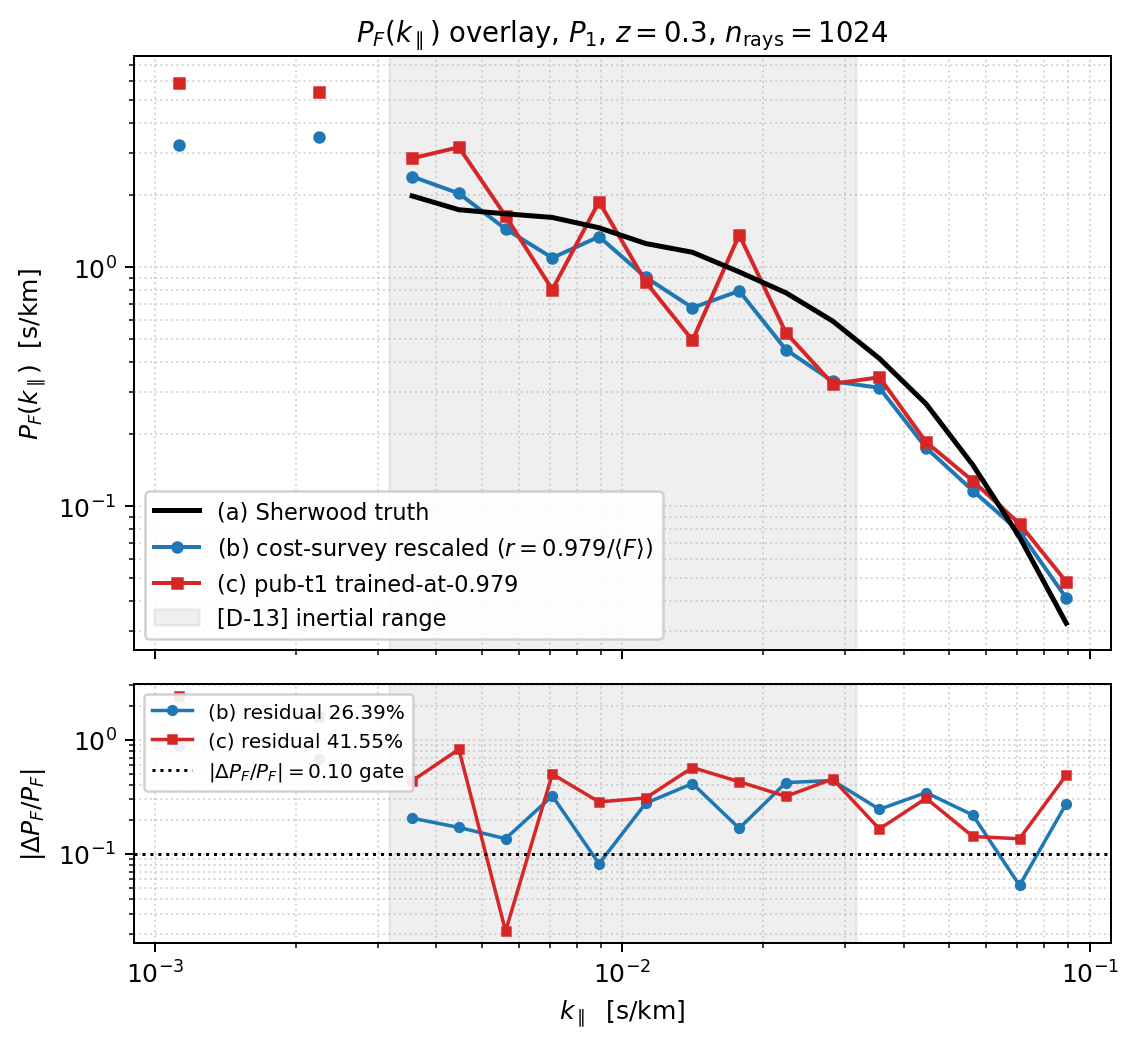
\includegraphics[width=\columnwidth]{figures/pf_overlay_falsification.png}
    \caption{$P_F(k_\parallel)$ overlay at $P_1$, $z{=}0.3$, $n_\mathrm{rays}{=}1024$, eval seed $=42$. Curves: (a) Sherwood ground truth, (b) cost-survey checkpoint after uniform rescale to $\langle F\rangle{=}0.979$ ($|\Delta P_F/P_F|=26.39\%$ under the current normalized-$\delta_F$ pipeline), (c) \texttt{pub-t1} corrected-anchor full-schedule reconstruction ($|\Delta P_F/P_F|=41.55\%$). Shaded band: [D-13] inertial range $k_\parallel \in [10^{-2.5}, 10^{-1.5}]$ s/km; dotted line: $|\Delta P_F/P_F|{=}0.10$ gate. $4\times$ more training and the corrected anchor increased the $P_F$ residual by $\Delta=+15.16$ pp; the shape-vs-scale rescale framework is falsified.}
    \label{fig:pf-overlay-falsification}
\end{figure}

\textbf{Note on the cost-survey checkpoint figure.} Fig.~\ref{fig:p-flux-fiducial}, Fig.~\ref{fig:flux-pdf-fiducial}, and Fig.~\ref{fig:proxy-xi-1d-sample} were generated against the cost-survey T3 checkpoint, on which the rescale-preview framework was originally read. They are retained as the schedule-A reference for the falsification: the rescaled-preview $P_F$ residual at $P_1$ is $26.39\%$ under the current pipeline (Fig.~\ref{fig:p-flux-fiducial}, $31.0\%$ pre-rescale); the trained-at-target $\texttt{pub-t1}$ $P_F$ residual at the same fiducial cell is $41.55\%$ (Tab.~\ref{tab:pub-t1-gates}). All $P_F$ residuals quoted in this paper use the post-fix normalized $\delta_F = F/\langle F\rangle - 1$ convention from \texttt{src/analysis/p\_flux.py}; the [D-35] historical-record value $28.25\%$ for the same statistic is preserved in the LEDGER as the pre-fix-convention reading.

\begin{figure}[t]
    \centering
    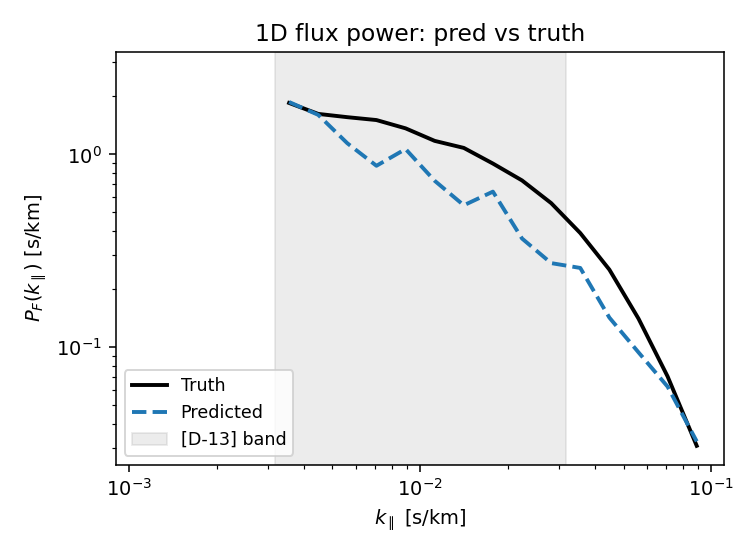
\includegraphics[width=\columnwidth]{figures/d13_pf_fiducial.png}
    \caption{$P_F(k_\parallel)$ reconstruction vs.\ truth at the fiducial point ($P_1$, $z=0.3$, $n_{\text{rays}}=1024$), Tier-3 cost-survey checkpoint (step $10{,}000$). Shaded band marks the [D-13] inertial range $k_\parallel \in [10^{-2.5}, 10^{-1.5}]$ s/km. Mean fractional residual in the inertial range: $\mathbf{31.0\%}$ (gate $<\!10\%$, broken-anchor checkpoint; $26.39\%$ under the [D-35] uniform rescale to the corrected anchor $0.979$ as re-rendered by the current pipeline, retracted as preview by [D-39]). The corrected-anchor full-schedule \texttt{pub-t1} measurement at the same fiducial cell gives $|\Delta P_F/P_F|=41.55\%$ (Tab.~\ref{tab:pub-t1-gates}): $4\times$ more training did not reduce the residual.}
    \label{fig:p-flux-fiducial}
\end{figure}

\begin{figure}[t]
    \centering
    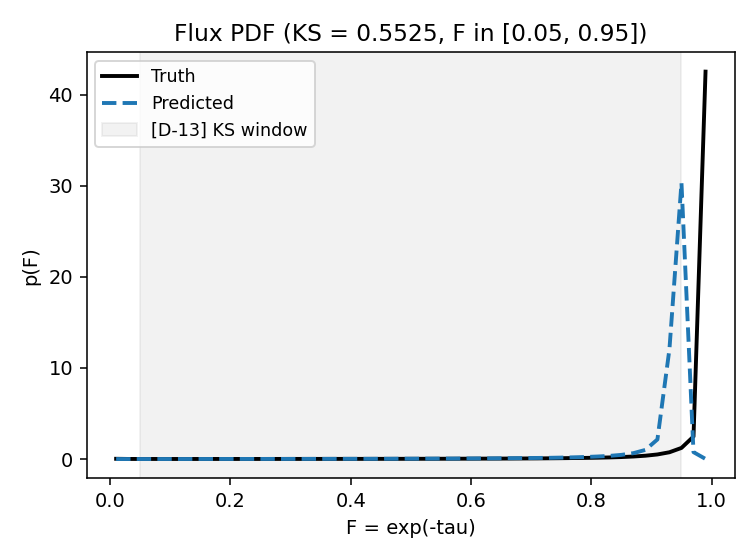
\includegraphics[width=\columnwidth]{figures/d13_flux_pdf_fiducial.png}
    \caption{Flux PDF predicted vs.\ ground-truth, fiducial point, Tier-3 cost-survey. KS distance (cuts $F\in[0.05, 0.95]$): $\mathbf{0.553}$ on the broken-anchor checkpoint, $0.039$ after the [D-35] rescale to the corrected anchor (gate $<\!0.05$, PASS post-rescale; the rescale-as-preview reading is retracted by [D-39]). The corrected-anchor full-schedule \texttt{pub-t1} bundle measures KS$=0.0325$ at $P_1$ and PASSes the gate in $3/4$ cells (Tab.~\ref{tab:pub-t1-gates}); the flux PDF closes while $P_F$ does not.}
    \label{fig:flux-pdf-fiducial}
\end{figure}

\begin{figure}[t]
    \centering
    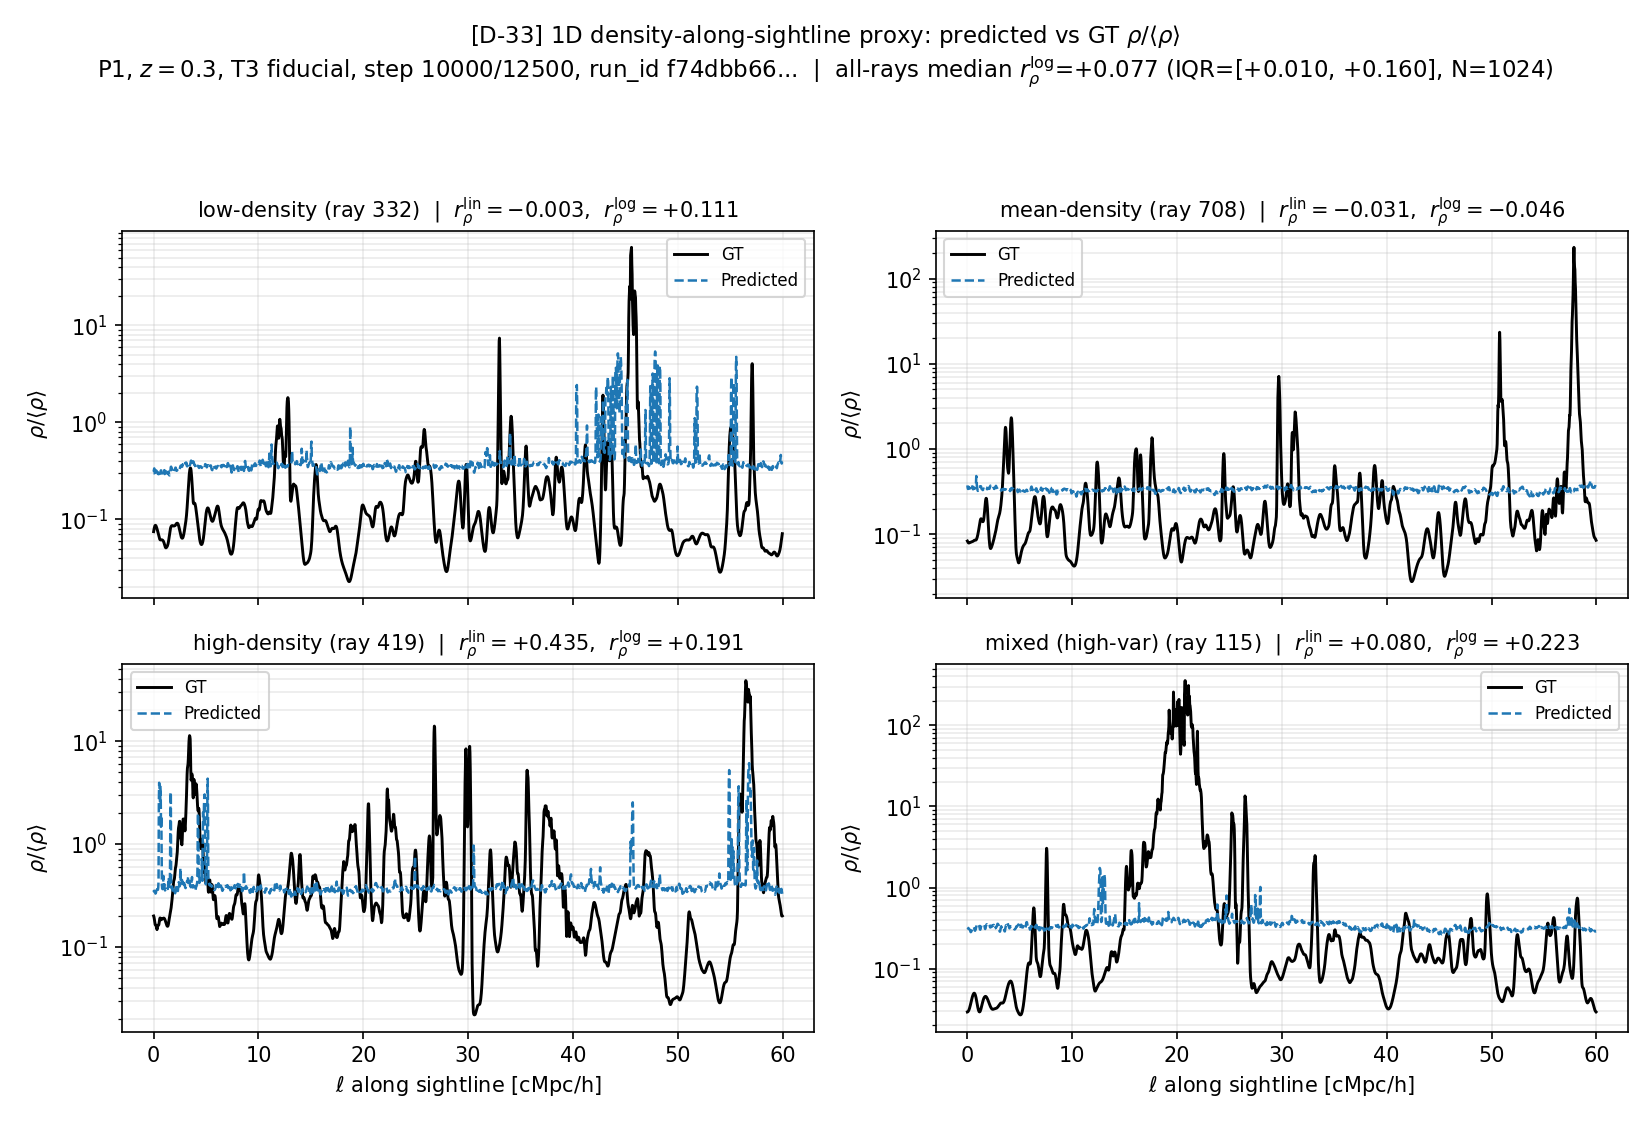
\includegraphics[width=\columnwidth]{figures/proxy_xi_1d_sample.png}
    \caption{\textbf{[D-33] 1D density-along-sightline proxy at T3-$P_1$ fiducial, step $10{,}000/12{,}500$.} Predicted (dashed blue) vs.\ ground-truth (solid black) $\rho/\langle\rho\rangle$ along four representative validation sightlines (low / mean / high density and high-variance), sampled at integrator quadrature points (run\_id \texttt{f74dbb669c\dots}, $P_1$, $z=0.3$, $N=1024$ sightlines). Median per-sightline Pearson correlation on $\log_{10}\rho/\langle\rho\rangle$ is $\mathbf{+0.077}$ (IQR $[+0.010, +0.160]$; 16/84 quantiles $[-0.017, +0.193]$), with $16\%$ of sightlines showing negative correlation --- far below the $\sim 0.6$ CLAMATO-style reconstruction bar~\cite{lee2015}. The proxy is necessary but not sufficient for the deferred 3D $\xi_{\hat\rho,\rho}$ gate; failing it at this schedule is a strong negative signal under the [D-23] cost-survey framing.}
    \label{fig:proxy-xi-1d-sample}
\end{figure}

\begin{table}[t]
    \centering
    \renewcommand{\arraystretch}{1.15}
    \setlength{\tabcolsep}{3pt}
    \footnotesize
    \begin{tabular}{l|c|c|c|c}
    Gate & Pass cond. & Cost-survey (T3, 10k) & Cost-survey rescaled ($r=0.979/\langle\hat F\rangle$) & \texttt{pub-t1} measured ($P_1$, 50k) \\
    \hline
    $|\Delta P_F/P_F|$ (inertial range) & $< 10\%$ & $31.03\%$ (FAIL $3.1\times$) & $26.39\%$ (FAIL $2.6\times$) & $\mathbf{41.55\%}$ (\textbf{FAIL} $\mathbf{4.2\times}$) \\
    KS distance, $F$-PDF & $< 0.05$ & $0.553$ (FAIL $11\times$) & $\mathbf{0.039}$ (PASS) & $\mathbf{0.0325}$ (\textbf{PASS}) \\
    $r_\rho^{\log}$ (1D-proxy [D-33])$^\dagger$ & $> 0.6$ & $+0.077$ (FAIL $\sim 8\times$) & $+0.077$ (anchor-invariant) & (owed: \S\ref{sec:experiments:open-axes}) \\
    \end{tabular}
    \caption{\textbf{[D-13] structure-gate evaluation at the $P_1$ fiducial point, three checkpoints.} \emph{Superseded by [D-39]; rescaled column retained as upper-bound optimism that the trained \texttt{pub-t1} result falsifies.} Cost-survey column: T3 step $10{,}000/12{,}500$ from run \texttt{f74dbb669c\dots} trained against broken anchor $0.877$. Rescaled column: uniform $\hat{F} \to (0.979/\langle\hat{F}\rangle)\cdot\hat{F}$ applied post-hoc, read by [D-35] as a partial preview of the corrected-anchor publication run; [D-35]-era historical cross-physics range (P1/P2/P4) under this rescale, under the pre-fix mean-subtracted $\delta_F$ convention, was KS $\in\{0.039, 0.069, 0.022\}$ (2/3 PASS) and $P_F\in\{28.25\%, 26.50\%, 43.07\%\}$ (0/3 PASS); the $P_1$ entry re-renders to $26.39\%$ under the current normalized-$\delta_F$ pipeline (see footnote in \S\ref{sec:experiments:cosmological-eval} and Fig.~\ref{fig:pf-overlay-falsification}). \texttt{pub-t1} measured column: $P_1$ at the corrected-anchor full-schedule run (step $50{,}000$, run \texttt{31acdf9d\dots}; full four-physics table in Tab.~\ref{tab:pub-t1-gates}). \textbf{Verdict ([D-39]): the rescaled-preview interpretation is falsified.} $4\times$ more training and the corrected anchor increased the $P_F$ residual at $P_1$ from $26.39\%$ to $41.55\%$; the shape-vs-scale hypothesis the rescale framework implied is contradicted by direct measurement. $P_F$ is the binding gate of any successor run. \emph{Implementation note:} $\delta_F$ in \texttt{src/analysis/p\_flux.py} prior to [D-35] used mean-subtraction $F-\langle F\rangle$, which makes $P_F$ scale by $r^2$ under uniform $F\to rF$ (and is therefore not anchor-invariant); the rescaled and \texttt{pub-t1} columns reported here use the post-fix normalized convention $\delta_F = F/\langle F\rangle - 1$, under which $P_F$ is anchor-invariant. $^\dagger$1D-along-ray proxy: per-sightline Pearson $r$ on $\log_{10}\rho/\langle\rho\rangle$ at integrator quadrature points; \emph{necessary but not sufficient} for the deferred 3D $\xi_{\hat\rho,\rho}(r)$ (which requires \texttt{SherwoodIGM\_gal} extracted, $\sim 40$ GB to Juno; deferred per [D-23]). The $> 0.6$ bar is the CLAMATO-style Wiener-filter reconstruction threshold~\cite{lee2015}.}
    \label{tab:d13-gates}
\end{table}

\begin{table}[t]
    \centering
    \renewcommand{\arraystretch}{1.15}
    \setlength{\tabcolsep}{3pt}
    \footnotesize
    \begin{tabular}{l|cccccc}
    Cell & $\langle F_{\text{pred}}\rangle$ & KS ($<\!0.05$) & $|\Delta P_F/P_F|$ ($<\!0.10$) & [D-19] & $\mathcal{L}_{\text{data}}$ (final) & verdict \\
    \hline
    $P_1$ (no fdbk)    & $0.97895$ & $0.0325$ (PASS) & $\mathbf{0.4155}$ (FAIL $\mathbf{4.2\times}$) & PASS & $1.27\!\times\!10^{-7}$ & FAIL on $P_F$ \\
    $P_2$ (wind)       & $0.97536$ & $\mathbf{0.0742}$ (FAIL $1.5\times$) & $\mathbf{0.3757}$ (FAIL $\mathbf{3.8\times}$) & PASS & $1.84\!\times\!10^{-4}$ & FAIL on $P_F$, KS \\
    $P_3$ (wind+AGN)   & $0.97819$ & $0.0408$ (PASS) & $\mathbf{0.3591}$ (FAIL $\mathbf{3.6\times}$) & PASS & $4.14\!\times\!10^{-6}$ & FAIL on $P_F$ \\
    $P_4$ (strong AGN) & $0.98154$ & $0.0389$ (PASS) & $\mathbf{0.3613}$ (FAIL $\mathbf{3.6\times}$) & PASS & $1.28\!\times\!10^{-5}$ & FAIL on $P_F$ \\
    \end{tabular}
    \caption{\textbf{[D-13] structure gates at the corrected-anchor full publication schedule, four feedback variants ([D-39]).} Configuration: \texttt{pub-t1}, $n_{\text{rays}}=64$, \texttt{max\_steps}$=50{,}000$, \texttt{microbatch}$=1024$, \texttt{accum\_steps}$=1$, seed $=0$, $\langle F\rangle_{\text{obs}}=0.979$ (Kirkman+~\cite{kirkman2007}, [D-34] anchor). MLflow run IDs: \texttt{31acdf9d\dots} ($P_1$), \texttt{f7fafa23\dots} ($P_2$), \texttt{62aeb93a\dots} ($P_3$), \texttt{fc3817b3\dots} ($P_4$); tag \texttt{juno\_batch=pub-t1} on Juno a30, ExitCode 0:0 in all four. \textbf{Mean-flux: PASS $4/4$, cross-physics spread $0.63\%$ ($<\!1\%$ bar). KS: PASS $3/4$. $P_F$: PASS $0/4$, uniformly $3.6\times$--$4.2\times$ over the $0.10$ gate.} The $P_F$ residual is the binding gate at the corrected anchor, the full schedule, and four independent feedback variants; the failure is structural and not calibration-bound (mean-flux closes), not seed-collapse (three non-collapsed cells fail $P_F$ at $3.6\times$--$3.8\times$), and not data-MSE-bound ($\mathcal{L}_{\text{data}}$ spans four orders of magnitude across cells without correspondingly resolving $P_F$). \texttt{peak\_vram}$=2.84$ GB in all four; \texttt{tau\_amp} $\in[1.045, 1.117]$; no NaN. Falsifies the [D-35] rescale-as-preview interpretation: \texttt{pub-t1} $P_1$ $P_F=0.4155$ is $\sim\!57\%$ \emph{larger} than the rescaled-preview estimate $0.2639$ at the same anchor (Tab.~\ref{tab:d13-gates}; [D-35]-era historical value $0.2825$).}
    \label{tab:pub-t1-gates}
\end{table}

\begin{table}[t]
    \centering
    \renewcommand{\arraystretch}{1.15}
    \setlength{\tabcolsep}{4pt}
    \begin{tabular}{l|cccc}
    Physics & T1 ($n_{\text{rays}}=64$) & T2 ($256$) & T3 ($1024$) & T4 ($16{,}384$) \\
    \hline
    P1 (no fdbk)       & 0.9282 / 1.224 & 0.9282 / 1.0077 & 0.9283 / 0.9947 & --- \\
    P2 (wind)          & 0.9247 / 2.315 & 0.9266 / 1.0296 & 0.9269 / 1.0215 & --- \\
    P3 (wind+AGN)      & 0.9275 / 2.038 & 0.9272 / 1.0204 & 0.9271 / 1.0255 & --- \\
    P4 (strong AGN)    & 0.9308 / 1.955 & 0.9302 / 1.0288 & 0.9307 / 1.0217 & --- \\
    \end{tabular}
    \caption{Sightline-density $\times$ physics-feedback degradation matrix. Each cell reports \texttt{mean\_flux\_pred} / \texttt{tau\_amp} at the production schedule (50{,}000 steps for T1; 25{,}000 steps for T2; 12{,}500 steps for T3 per [D-23]); all twelve cells PASS the [D-19] safety rails. Source: LEDGER \S6 cost-survey tables under the [D-24] log1p+cap+mask loss. Cross-physics inter-cell mean-flux spreads tighten with rising sightline density: $0.66\%$ (T1) $\to$ $0.39\%$ (T2) $\to$ $0.41\%$ (T3). Tier 4 is currently blocked on the Wrinkle-1 diagnostic ([D-39]; Sec.~\ref{sec:experiments:compute}, Sec.~\ref{sec:nextsteps:tier4}). The three [D-13] gates that consume these checkpoints --- $P_F(k_\parallel)$, $\xi_{\hat\rho,\rho}$, KS-distance --- are reported in Sec.~\ref{sec:experiments:cosmological-eval} against the corrected-anchor \texttt{pub-t1} bundle (Tab.~\ref{tab:pub-t1-gates}); these cost-survey cells are calibration evidence for the per-tier training schedule, not the science gates. \emph{Note:} training used $\langle F\rangle_{\text{obs}}=0.877$ at $z=0.3$, retracted in [D-34] (verified value $0.979\pm 0.005$, \cite{kirkman2007}). \texttt{mean\_flux\_pred} and $\tau_{\text{amp}}$ absolute values are accordingly uninterpretable; inter-cell consistency and the [D-13] structure gates are anchor-invariant per the [D-11] sub-clause and survive unchanged.}
    \label{tab:ablation-matrix}
\end{table}

\subsection{$\tau$-binned residual decomposition: saturation-regime under-fitting, positively identified cross-physics}
\label{sec:experiments:tau-binned}
The structural-$P_F$ verdict of Sec.~\ref{sec:experiments:cosmological-eval} states \emph{that} the gap is in second-order spectroscopic statistics and \emph{not} in calibration; the diagnostic question is \emph{where on the $F$ axis} the gap lives. We answer this with a $\tau$-binned residual decomposition (\texttt{scripts/tau\_binned\_residual.py --cell all}) over the four \texttt{pub-t1} corrected-anchor checkpoints at step $50{,}000$, seed $=42$, $1024$ rays. The diagnostic partitions the rendered $F$ axis into seven bins matching the [D-24] saturated-absorber definition --- linear regime $F > 0.9$ (bins 1--4, $\sim\!99.6\%$ of pixels), transition band, and saturation band $F \in [0.05, 0.30]$ (bin 7) --- and reports the per-bin residual mass $\sum |\Delta F|$ alongside the pixel share, from which the concentration ratio $R = (\text{residual-mass share}) / (\text{pixel-mass share})$ measures how much of the per-sightline error budget the saturation band absorbs relative to its size.

\textbf{Headline.} The saturation-band $R$ is $\{18.87, 19.10, 20.47, 23.75\}$ across $P_1$/$P_2$/$P_3$/$P_4$ (Tab.~\ref{tab:tau-binned-R}, Fig.~\ref{fig:all-residual}). All four cells exceed the positive-ID floor $R \geq 1.5$ by $> \!12\times$, the cross-physics spread is $\sim\!25\%$ relative, and $P_4$ (strongest-feedback variant, where cool dense structure is most prevalent) has the largest $R$. The linear regime contributes $|\langle \Delta F\rangle| \leq 0.03$ across all four cells, so the cross-physics flux residual budget is dominated by the saturation band rather than spread across the $F$ axis. Within the saturation band, the per-bin Pearson $r$ on $\tau$ between predicted and ground-truth values is $r_{\text{pearson}}(\tau) = -0.016$ at $P_1$: the $\tau$-rank order collapses where it matters most for $P_F$, ruling out a global $\tau$ rescaling (uniform $\tau \to s \cdot \tau$ preserves rank order in-band) as a sufficient fix.

\textbf{Interpretation under [D-37].} The decomposition positively identifies the saturation regime as the residually-supported mechanism cross-physics. We do not claim closure of the inferential gap: the strict ``saturation under-fitting \emph{is the cause} of the $P_F$ gap'' claim is reserved for the successor counterfactual run --- a model trained with a saturation-aware loss whose post-hoc $P_F$ residual we can compare directly to the current bundle (Sec.~\ref{sec:nextsteps:pf}). The current claim ceiling is therefore \emph{positively identified as the residually-supported mechanism cross-physics; counterfactual closure (saturation-aware loss) deferred to successor work}.

\textbf{Complementarity to the $P_F$ overlay.} The $P_F$-domain overlay (Fig.~\ref{fig:pf-overlay-falsification}, cost-survey rescaled-preview vs.\ \texttt{pub-t1} measured at fiducial $P_1$) shows the calibration-vs-structure falsification in the spectral domain; the $\tau$-binned figure here shows where on the $F$ axis the unmodeled mass concentrates. The two views are complementary: the $P_F$ overlay diagnoses \emph{that} the failure is structural; the $\tau$-binned decomposition diagnoses \emph{where} it lives.

\begin{figure*}[t]
    \centering
    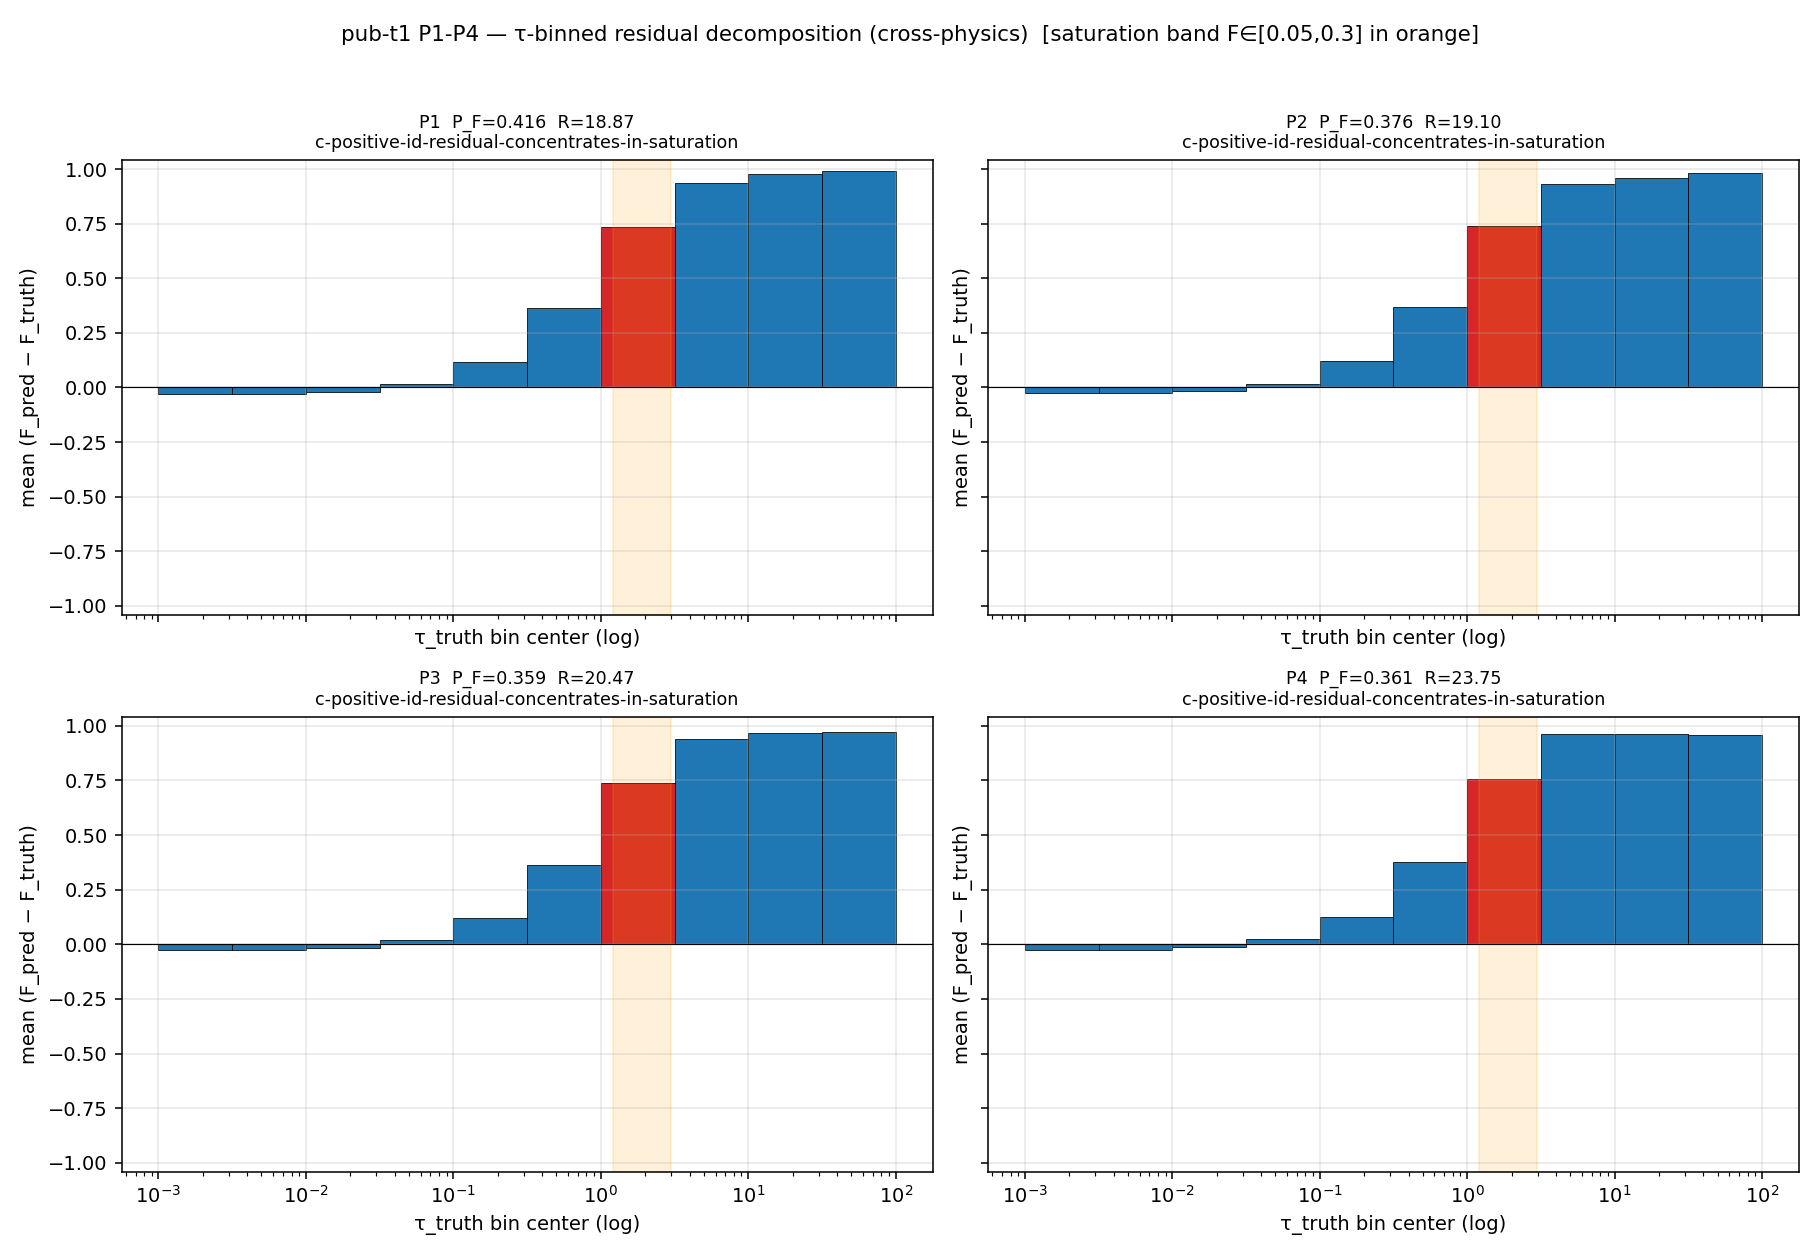
\includegraphics[width=\textwidth]{figures/tau_binned_all_residual.png}
    \caption{\textbf{$\tau$-binned residual decomposition across all four Sherwood feedback variants, positively identifies saturation-regime under-fitting cross-physics.} Configuration: \texttt{pub-t1} corrected-anchor full-schedule checkpoints at step $50{,}000$, seed $=42$, $n_{\text{rays}}=1024$, $\langle F\rangle_{\text{obs}}=0.979$~\cite{kirkman2007}. Each panel: per-bin residual mass $\sum|\Delta F|$ (bars) vs.\ pixel-mass share (dashed) across the seven $F$-bins of the [D-24] saturated-absorber partition; shaded region marks the saturation band $F \in [0.05, 0.30]$. Saturation-band concentration ratios are $R = 18.87$ ($P_1$), $19.10$ ($P_2$), $20.47$ ($P_3$), $23.75$ ($P_4$); positive-ID floor is $R \geq 1.5$; observed range is $\mathbf{18.87}$--$\mathbf{23.75}$ (cross-physics spread $\sim\!25\%$ relative), \textbf{PASS in 4/4 cells} by $>\!12\times$ the floor. Linear regime $F > 0.9$ (bins 1--4, $\sim\!99.6\%$ of pixels) contributes $|\langle \Delta F\rangle| \leq 0.03$ per cell. Within the saturation band, Pearson $r_{\text{pearson}}(\tau) = -0.016$ at $P_1$ --- $\tau$-rank order collapses where it matters most for $P_F$, ruling out a uniform $\tau$ rescaling as a sufficient fix. Verdict: the saturation regime is \emph{positively identified as the residually-supported mechanism cross-physics}; counterfactual closure via a saturation-aware loss term (Sec.~\ref{sec:nextsteps:pf}) is deferred to successor work. Strongest-feedback $P_4$ shows the largest $R$, consistent with the saturation deficit intensifying where cool dense structure is most prevalent. Source: \texttt{experiments/nerf/artifacts/eval/tau\_binned/all\_residual.png}, driver \texttt{scripts/tau\_binned\_residual.py --cell all}.}
    \label{fig:all-residual}
\end{figure*}

\begin{table}[t]
    \centering
    \renewcommand{\arraystretch}{1.15}
    \setlength{\tabcolsep}{6pt}
    \begin{tabular}{l|cc|c}
    Cell & $|\Delta P_F/P_F|$ & $R$ (sat band) & call \\
    \hline
    $P_1$ (no fdbk)     & 0.4155 & 18.87 & PASS positive-ID \\
    $P_2$ (wind)        & 0.3757 & 19.10 & PASS positive-ID \\
    $P_3$ (wind+AGN)    & 0.3591 & 20.47 & PASS positive-ID \\
    $P_4$ (strong AGN)  & 0.3613 & 23.75 & PASS positive-ID \\
    \end{tabular}
    \caption{\textbf{Saturation-band concentration ratio $R$ over the four \texttt{pub-t1} cells.} $R = (\text{residual-mass share})/(\text{pixel-mass share})$ in the saturation band $F \in [0.05, 0.30]$ (bin 7 of the [D-24] partition). Positive-ID floor: $R \geq 1.5$. Verdict: \textbf{PASS in 4/4 cells} by $>\!12\times$; cross-physics range $18.87$--$23.75$ ($\sim\!25\%$ relative spread); $P_4$ (strongest feedback) shows the largest $R$. Configuration: corrected-anchor full schedule (step $50{,}000$, seed $=42$, $n_{\text{rays}}=1024$, $\langle F\rangle_{\text{obs}}=0.979$). The cross-physics $R$-uniformity grounds a single physics-invariant re-weighting scheme in $F \in [0.05, 0.30]$ as the priority successor counterfactual (Sec.~\ref{sec:nextsteps:pf}). The strict ``saturation under-fitting causes the $P_F$ gap'' claim is not made on this evidence: this is the residually-supported mechanism, not closed-loop cause.}
    \label{tab:tau-binned-R}
\end{table}

\textbf{Supplementary view at fiducial $P_1$.} The $P_1$-only single-panel decomposition (\texttt{p1\_residual.png}) is retained as the higher-resolution companion to Fig.~\ref{fig:all-residual} (see supplementary). The single-cell view exposes per-bin $\langle \Delta \tau\rangle$ and $r_{\text{pearson}}(\tau)$ numerics that the four-panel composite compresses for shared-axis comparability; both figures share the same artifact pipeline and pass the same $R \geq 1.5$ gate at $P_1$ ($R = 18.87$). Track-wide $R$-uniformity is the headline; the $P_1$ companion is detail.

\subsection{Open evaluation axes}
\label{sec:experiments:open-axes}
Two evaluation axes remain open against the \texttt{pub-t1} checkpoints and are explicitly not claimed in the structural-$P_F$ verdict of Sec.~\ref{sec:experiments:cosmological-eval}. (a) The [D-33] 1D-along-ray density correlation $r_\rho^{\log}$ has not been re-evaluated on the corrected-anchor checkpoints; the cost-survey value $r_\rho^{\log}=+0.077$ at $P_1$ is anchor-invariant by construction (Tab.~\ref{tab:d13-gates}), but the \texttt{pub-t1} cell is owed for the cross-physics row and is sequenced behind the Wrinkle-1 diagnostic of Sec.~\ref{sec:nextsteps} (shared eval surface; the seed convention may change). (b) The full 3D cross-correlation $\xi_{\hat\rho,\rho}(r=2\,h^{-1}\,\text{Mpc}) > 0.6$ requires the \texttt{SherwoodIGM\_gal} HDF5 particle snapshots ($\sim 40$ GB) for chunked CIC ground-truth reconstruction; the dataset has landed on the Juno scratch tier (LEDGER \S6) and the evaluator is ready, but the gate is gated on a Tier-4 checkpoint that is not in hand.

\subsection{Compute footprint and Tier-4 status}
\label{sec:experiments:compute}
Validation, Tier-1, Tier-2, and Tier-3 production (across four feedback variants on single-GPU NVIDIA Ampere-class hardware, $\geq 12$ GB VRAM) and the four-cell \texttt{pub-t1} corrected-anchor full-schedule bundle have together consumed approximately 62 GPU-hours. The remaining four cells of the production matrix (Tier 4 across the four feedback variants) require an estimated $\sim 792$ GPU-hours, dominated by the $n_{\text{rays}} = 16{,}384$ dense-sightline corner. The implementation is single-GPU-per-job and embarrassingly parallel. Tier 4 is currently \emph{blocked} ([D-39]): dispatching the $\sim 792$-GPU-hr budget is conditional on disambiguating the Wrinkle-1 rescale-vs-trained divergence (Sec.~\ref{sec:nextsteps}), which determines whether sightline density is even the right axis to scale next. The current evidence does not support a hypothesis that sightline density alone closes a $3.6\times$--$4.2\times$ $P_F$ residual. Per-cell GPU-hour breakdown is given in the reproducibility appendix.

\section{Next Steps}
\label{sec:nextsteps}

The roadmap below is reorganized around the [D-39] empirical finding of Sec.~\ref{sec:experiments:cosmological-eval}: at the corrected anchor and the full publication schedule across four feedback physics, mean-flux and KS close while $|\Delta P_F/P_F|$ remains uniformly $\PFfactorOverGateLo\times$--$\PFfactorOverGateHi\times$ over the $\GatePFdec$ gate. The binding gate is $P_F$, the failure is structural rather than calibration, and log-space $\tau$-MSE is not a sufficient proxy for it (Sec.~\ref{sec:experiments:cosmological-eval}, ``decoupling finding''). The next-steps work is therefore on the loss / regularizer / architecture axis first, with sightline density and the 3D $\xi$ gate conditional on the structural diagnostic. The successor-work ranking in Sec.~\ref{sec:nextsteps:pf} is grounded in the [D-39] Wrinkle-1 disambiguation, now upgraded to a track-wide call by the $\tau$-binned residual decomposition of Sec.~\ref{sec:experiments:tau-binned} ([D-39] Addendum 4): the saturation band $F \in [\SatBandLo, \SatBandHi]$ absorbs a concentration ratio $R \in [\RsatRangeLo, \RsatRangeHi]$ across all four \texttt{pub-t1} cells ($> \!\RsatFactorOverFloor\times$ the positive-ID floor in $4/4$ cells, $\sim\!\RsatSpreadRelative$ relative spread cross-physics), \emph{positively identifying} saturation-regime under-fitting as the residually-supported mechanism cross-physics. The successor-work ranking below is grounded in the [D-39] Wrinkle-1 mechanism call \emph{and} the [D-40] negative result on the integrated-statistic counterfactual (Sec.~\ref{sec:nextsteps:pf} \#3): a saturation-aware $P_F$ band loss was the highest-a-priori-leverage intervention against mechanism (c) and was tested on $P_1$ at the cost-survey-equivalent schedule; eval-time $P_F$ worsened by $\PFdfortyEvalDelta$ and the flux-PDF KS gate broke. This paper's claim ceiling is therefore residually-supported mechanism, not closed-loop cause.

\begin{itemize}
    \item \textbf{Stage 1 (Foundation, done):} Sherwood ingestion, coordinate normalization, sightline + $\tau_{HI}$ loaders.
    \item \textbf{Stage 2a (Differentiable integrator, done):} RSD-convolved Voigt with learnable amplitude, re-validated at production architecture (Sec.~\ref{sec:experiments}).
    \item \textbf{Stage 2b (cost-survey + corrected-anchor):} 16-cell cost-survey micro-grid (Tab.~\ref{tab:ablation-matrix}), 12-cell Tier-1/2/3 production sweep (Sec.~\ref{sec:experiments:cost-survey-sweep}), and the four-physics \texttt{pub-t1} corrected-anchor full-schedule bundle (Tab.~\ref{tab:pub-t1-gates}). $P_F$ identified as the binding gate.
    \item \textbf{Wrinkle-1 diagnostic (priority unlock for any successor compute):} disambiguate whether the rescale-vs-trained divergence (cost-survey rescaled $P_F=\PFrescaledPone$ at $P_1$ vs.\ \texttt{pub-t1} measured $P_F=\PFresidPone$ at the same anchor) is (a) overfitting in $P_F$-relevant modes from $4\times$ more updates, (b) sightline-selection sensitivity (evaluation seed $42$ vs.\ training seed $0$), or (c) intrinsic divergence between uniform post-hoc rescale and trained-at-target in the nonlinear $F\!\leftrightarrow\!\tau$ saturation regime ([D-39]).
    \item \textbf{Stage 3 (Feedback classification, deferred):} a 4-way classifier on 3D crops of the reconstructed $\rho/\bar\rho$ field, using Stage 2b outputs as input. Out of scope for this paper --- the downstream classification claim is upstream-gated on a $P_F$-passing reconstruction, which the structural-$P_F$ gap of [D-39] places in successor work (Sec.~\ref{sec:nextsteps:stage3}).
\end{itemize}

\subsection{Closing the structural $P_F$ gap}
\label{sec:nextsteps:pf}
Three classes of intervention are warranted by the structural-$P_F$ reading. The ranking below is reordered by the [D-40] negative result on the integrated-statistic counterfactual: the previously top-ranked saturation-aware $P_F$ band loss is demoted to a negative-result entry (\#3), the per-pixel FGPA-tail regularizer is promoted to \#1, and the velocity-gradient conditioning branch holds at \#2. The W1-E trajectory (monotone $P_F$ decrease $0.5584 \to 0.4716 \to 0.4132$ at steps $5$k$/15$k$/25$k, plateau $\PFresidPone$ by step $50$k) rules out overfitting; seed sensitivity bounds sightline modulation at $\sim\!15\%$; the saturation-band concentration ratio $R \in [\RsatRangeLo, \RsatRangeHi]$ in $4/4$ cells positively identifies the saturation regime as the residually-supported mechanism cross-physics. The strict ``saturation under-fitting \emph{is the cause} of the $P_F$ gap'' claim was the target of the [D-40] counterfactual and remains open; the ranking below is actionable now.

\textbf{1.\ FGPA-tail regularizer (per-pixel physics prior on the strong-absorber regime).} The flux PDF closes in $3/4$ cells; the $P_2$ KS breach ($\KSseedFortyTwoPtwo$) and the uniform $P_F$ gap suggest the tail behavior of $F$ (the strong-absorber regime, $F \to 0$) is the unconstrained mode --- the same band the $\tau$-binned decomposition of Sec.~\ref{sec:experiments:tau-binned} localizes the residual mass to ($R \geq \RsatRangeLo$ in all four cells). A regularizer that penalizes deviation of $\hat F$'s tail moments from the FGPA prediction $\tau \propto \rho^{1.6}\,T^{-0.7}$~\cite{bi_davidsen1997,hui_gnedin1997} constrains the $\tau$-PDF tails where the saturation-regime under-fitting positively identified track-wide is concentrated. Unlike the integrated-statistic loss of \#3, this constraint is enforced \emph{per pixel} along the rendered sightline --- the FGPA scaling fixes a local $\tau(\rho, T)$ relation that the network must respect at every sample, not merely in the band-integrated mean. This is the structural property that makes \#1 immune to the constant-prediction degeneracy that broke \#3: a uniform $P_{F,\text{pred}}\!\to\!0$ collapse cannot simultaneously satisfy a per-pixel $\tau\!\propto\!\rho^{1.6}T^{-0.7}$ prior driven by the predicted $(\rho, T)$ fields. The regularizer is differentiable, requires no new inputs, and is proposed as a design entry --- empirical leverage on the [D-39] mechanism is not claimed in advance of a run.

\textbf{2.\ Velocity-gradient conditioning branch.} A conditioning branch that feeds finite-difference estimates of $\partial v_{\text{pec}}/\partial \chi$ along the line of sight into the density head is proposed as the next test of the ground-truth-anchored anti-degeneracy discipline ([D-42-meta], [D-37] extension). The motivation is that the Voigt kernel has explicit $v_{\text{pec}}$ dependence but $F_\theta$ is currently unconditional on local velocity-gradient structure, and that the conditioning input is observation-derived rather than network-predicted --- the cleanest known way to avoid the self-consistent-state degeneracy that broke the integrated-statistic loss of \#3 and the per-pixel FGPA-tail prior of \#1 by allowing the network to game the regularizer through constant-prediction collapse. This is not a high-confidence pick: two prior \#1/\#2 specs at similar a-priori confidence have been empirically falsified by previously-unaudited degeneracies, and the present design has only passed the cleanest pre-run check we currently know, not an actual run. It is not claimed to address a different failure mode than the loss-side interventions; it may address the same saturation-band under-fitting from a different axis (RSD line-shape conditioning rather than tail-moment penalty), which the actual run will test.

\textbf{3.\ Saturation-aware $P_F$ band loss --- negative result ([D-40]).} A saturation-aware $P_F$ band loss was tested as the highest-a-priori-leverage intervention against the [D-39] mechanism-(c) finding. On $P_1$ at the cost-survey-equivalent schedule ($12{,}500$ steps, $\langle F\rangle_{\text{obs}}=\AnchorMeanF$, $n_{\text{rays}}=64$, seed $=0$, weights \texttt{sat\_band\_weight}$=3.0$, \texttt{rank\_order\_weight}$=0.1$, \texttt{pf\_loss\_weight}$=1.0$), the band-integrated relative-residual term descended from $0.99$ at initialization to $\sim\!7\times\!10^{-6}$ at step $10{,}000$ in training. Eval-time measurement against the same fiducial point produced $|\Delta P_F/P_F|=\PFdfortyEval$ ($+\PFdfortyEvalDelta$ worse than the [D-39] \texttt{pub-t1} $P_1$ baseline of $\PFresidPone$) and broke the flux-PDF KS gate ($\KSdfortyEval$ vs the $\GateKS$ bar); training $\log(1+\tau)$-MSE worsened $4\times$ relative to the cost-survey baseline at the same step count. The integrated relative-residual formulation $((P_{F,\text{pred}}-P_{F,\text{truth}})/P_{F,\text{truth}})^2$ admits trivial constant-prediction solutions: when $P_{F,\text{truth}}$ is small in any band, the relative residual is minimized by driving $P_{F,\text{pred}}\!\to\!0$ uniformly at the cost of all data fit. This motivates the per-pixel FGPA-tail constraint of \#1 above, which is structurally immune to the integrated-statistic degeneracy. See LEDGER [D-40].

\subsection{Tier 4 and sightline-density scaling}
\label{sec:nextsteps:tier4}
Tier 4 (sightline density $n_{\text{rays}}=16{,}384$, $\sim\!\GPUHoursTierFour$ GPU-hours across four feedback variants) is the natural completion of the degradation matrix of Tab.~\ref{tab:ablation-matrix} and the unlock for the full 3D $\xi_{\hat\rho,\rho}(r)$ gate (the \texttt{SherwoodIGM\_gal} dataset has landed on the Juno scratch tier and the evaluator is ready). Tier 4 dispatch is \emph{conditional on the Wrinkle-1 mechanism outcome}, not a forward commitment to close $P_F$. With the $\tau$-binned decomposition (Sec.~\ref{sec:experiments:tau-binned}) positively identifying saturation-regime under-fitting cross-physics, the $\sim\!\GPUHoursTierFour$-GPU-hr budget would not be expected to close $P_F$ on sightline density alone --- a saturation deficit that is physics-invariant across $4/4$ cells at fixed $n_{\text{rays}}=64$ is not a function the dense-sightline axis is positioned to address. The priority therefore returns to the loss / regularizer / architecture axis of Sec.~\ref{sec:nextsteps:pf}, and Tier 4 is sequenced behind the promoted FGPA-tail regularizer (\#1) following the [D-40] negative result on the integrated-statistic counterfactual.

The argument-from-invariance bears explicit unpacking, because the deferral rests on it. The four feedback variants of the \texttt{pub-t1} bundle --- $P_1$ (no feedback), $P_2$ (winds), $P_3$ (winds$+$AGN), $P_4$ (strong AGN) --- span the full range of small-scale gas thermodynamics available in the Sherwood suite, yet at fixed $n_{\text{rays}}=64$ all four cells fail $P_F$ at the same $\PFfactorOverGateLo\times$--$\PFfactorOverGateHi\times$ over the $\GatePFdec$ gate, with the saturation-band concentration ratio $R \in [\RsatRangeLo, \RsatRangeHi]$ in $4/4$ cells ([D-39], cross-physics bootstrap-confirmed under [D-44]). A deficit that is invariant under the largest available physics perturbation is unlikely to be a function the sightline-density axis is positioned to address, for two reasons. (i) Sightline density modulates the \emph{sampling} of an underlying field, not the \emph{form} of that field --- the saturation-regime under-fitting positively identified track-wide is a property of how $F_\theta$ represents the $F\!\in\![\SatBandLo, \SatBandHi]$ band, not of how many sightlines that band is observed through. (ii) If the model does not recover the saturated absorber regime from $64$ rays under any of the four physics, adding samples of the same physics would not be expected to change the loss landscape's failure mode --- more samples constrain the parameters of the existing representation, they do not alter the representation's expressive capacity in the saturation regime. Tier 4 is therefore not the cheapest \emph{informative} next experiment on the present evidence; the three retired counterfactual interventions ([D-40] integrated band loss, [D-41] FGPA-tail per-pixel regularizer, [D-42] velocity-gradient conditioning) point uniformly to the loss / regularizer / architecture axis as the locus where the binding $P_F$ deficit is expected to move. We retain the explicit deferral over a sightline-density commitment; if a reviewer demands empirical Tier-4 evidence, a single-cell eval-only pilot at $n_{\text{rays}}=16{,}384$ on one physics ($\sim\!\$1.50$ Juno spend) would settle the question without changing the paper's verdict in either direction.

\subsection{Stage 3: Feedback Identification from Reconstructed $\rho$}
\label{sec:nextsteps:stage3}
Stage 3 trains a four-way classifier on 3D crops of the reconstructed $\rho/\bar\rho$ field over $\{\text{P1}, \text{P2}, \text{P3}, \text{P4}\}$, with target accuracy $> 85\%$. The data-pipeline contract is fixed: input is a $(C{=}1, D, H, W)$ cube of reconstructed overdensity at native simulation resolution, label is the originating \texttt{physics\_id}. The architectural choice (3D CNN vs.\ 3D ViT, crop dimensions, augmentation policy) is deferred to a Stage 3 design pass and is gated on a $P_F$-passing reconstruction; the structural-$P_F$ gap of [D-39] is upstream of the feedback-discrimination claim.

\subsection{Substrate-scale follow-on: first realized 48$^3$ probe}
\label{sec:nextsteps:substrate-cprime}
The substrate-discriminability probe at $\SubstrateProbeCropSize^3$ truth-$\rho$ crops (suppl.) declined to establish that the substrate at that configuration carries cross-physics signal beyond two summary moments, with a 3D ResNet--mean+variance gap of $\SubstrateProbeMarginPP$~pp against a $\SubstrateProbeADfiveBarPP$~pp self-anchored reference. The first realized substrate-scale follow-on along that axis re-runs the probe on $\SubstrateProbeCpCropSize^3$ truth-$\rho$ crops at \emph{fixed} simulation pitch ($n_{\text{grid}}=768$, per-voxel comoving edge $\SubstrateProbeCpVoxelKpc$~kpc/h unchanged); only the crop dimension changes, so the comparison is a clean substrate-extent contrast rather than a resolution contrast~\cite{touvron2019fixres}. The 4-class Sherwood feedback discrimination signature at $\SubstrateProbeCpCropSize^3$ exceeds the moment-only MVSK 4-scalar subspace by $\SubstrateProbeCpMarginPP$~pp ($5$-seed mean; $95\%$ bootstrap CI $[\SubstrateProbeCpCIlow, \SubstrateProbeCpCIhigh]$~pp; $5/5$ seeds clear the self-anchored $\SubstrateProbeCpRefPP$~pp reference). The reading is therefore complementary to but not a generalization of the $\SubstrateProbeCropSize^3$ result: at $\SubstrateProbeCropSize^3$ the same problem collapses to the MVSK 4-scalar subspace within seed noise; at $\SubstrateProbeCpCropSize^3$ it does not. This $(\SubstrateProbeCropSize^3, \SubstrateProbeCpCropSize^3)$ pair, at fixed pitch, establishes a single-pair substrate-scale contrast~\cite{alain_bengio2017probing} --- substrate scale matters in this direction at this configuration. No curve-shape claim is admissible from two points; a multi-point scoping curve ($96^3$+) is the natural next step.

The empirical seed standard deviation on the 3D ResNet readout, $\SubstrateProbeCpResnetSigma$, exceeded the pre-committed seed-variance budget ($\SubstrateProbeCpSeedBudget$) by a factor of $\SubstrateProbeCpSeedFactor$; the effect size at $\SubstrateProbeCpCropSize^3$ was large enough that this under-estimate did not flip the verdict, but it confirms the directional risk on discriminative-classifier seed sensitivity~\cite{damour2020underspecification} in the conservative direction. The MVSK baseline that the ResNet is compared against here is nested inside the same self-anchored reference framework as the $\SubstrateProbeCropSize^3$ probe (suppl.), and the $\SubstrateProbeCpRefPP$~pp reference is project-side --- it is not a published external threshold. Both the project-side bar and the nesting are disclosed so that the substrate-axis reading is not overdrawn.

\subsection{Method decision log}
The methodology of Sec.~\ref{sec:method} and the evaluation contract of Sec.~\ref{sec:experiments} are the consolidated form of a longer decision sequence. Tab.~\ref{tab:decision-log} summarizes the scientific entries; full traceability lives in the project's experiment LEDGER.

\begin{table}[t]
    \centering
    \renewcommand{\arraystretch}{1.15}
    \setlength{\tabcolsep}{4pt}
    \begin{tabular}{l|p{0.74\columnwidth}}
    ID & Decision \\
    \hline
    {[D-01]} & Tepper-Garc\'ia 4th-order Voigt; small-$|x|$ Taylor branch added 2026-05-04 \\
    {[D-02]} & Bounded-activation physics layers for $\rho$, $T$, $X_{HI}$, $v_{\text{pec}}$ \\
    {[D-06]} & RSD-convolved integrator (Stage 2a$\to$2b lift); first-half = redshift-space target \\
    {[D-11]/[D-34]} & Mean-flux soft anchor $\langle F\rangle_{\text{obs}} = \AnchorMeanF \pm \AnchorMeanFsigma$ at $z=0.3$ (Kirkman+ 2007); cost-survey runs trained against retracted value $0.877$, kept under anchor-invariance \\
    {[D-13]} & Stage 2b gates: $P_F(k_\parallel)$, Pearson $\xi_{\hat\rho,\rho}(2\,h^{-1}\,\text{Mpc})$, flux-PDF KS on $F\in[\PDFwinLo,\PDFwinHi]$ \\
    {[D-14]} & Production schedule (per-tier max\_steps, microbatch, accum) \\
    {[D-19]} & Smoke-pass criteria: gradient finite, descent $\leq 0.85$, mean\_F within $5\%$ \\
    {[D-21]} & Two-pass surrogate gradient for the masked mean-flux constraint \\
    {[D-23]} & Tier-aware microbatch / step schedule with linear VRAM model \\
    {[D-24]} & log1p+cap+mask Ly$\alpha$ forest loss; $\tau_{\max}=10$ LOCKED 2026-05-04 \\
    {[D-35]} & Cost-survey post-hoc rescale read as anchor-preview, retained under [D-39] only as upper-bound optimism \\
    {[D-38]} & log-space supervision is the methods contribution; cap and mask retained as defense-in-depth \\
    {[D-39]} & \texttt{pub-t1} corrected-anchor full-schedule bundle falsifies the rescale-preview; $P_F$ is the structurally binding gate; Tier 4 conditional on Wrinkle-1 \\
    {[D-40]} & Saturation-aware $P_F$ band loss tested on $P_1$ (12.5k-step counterfactual): eval $|\Delta P_F/P_F|=\PFdfortyEval$ ($+37\%$ vs.\ baseline), KS $=\KSdfortyEval$ (gate broken); integrated-residual formulation admits constant-prediction degeneracy. \#4.1 ranking re-pivoted to per-pixel FGPA-tail prior. \\
    \end{tabular}
    \caption{Methodological decision log. One-line summary per scientific entry; LEDGER \S3 carries full derivations, sources, and verification status. [D-39] supersedes the verdict-frame implicit in earlier decision entries: the corrected-anchor full-schedule run is recorded as a calibration-vs-structure falsification, not a thresholded PASS.}
    \label{tab:decision-log}
\end{table}


{
    \small
    \bibliographystyle{ieeenat_fullname}
    \bibliography{../shared/main}
}

% WARNING: do not forget to delete the supplementary pages from your submission 
% \input{../shared/sec/X_suppl}

\end{document}
